\documentclass[12pt]{report}
\usepackage[a4paper,left=25mm, right=25mm, top=30mm, bottom=30mm]{geometry}
\usepackage[english]{babel}
\usepackage[utf8x]{inputenc}
\usepackage{amsmath}
\usepackage{graphicx}
\usepackage{wrapfig}
\usepackage{microtype}
\usepackage{setspace}
\usepackage{enumitem}
\usepackage{booktabs}
\usepackage{subfig}
\usepackage[nottoc]{tocbibind}
\usepackage{natbib}
\usepackage[section]{placeins}
\usepackage{multicol}
\usepackage{graphicx}
\usepackage{lscape}
\usepackage{amssymb}
\usepackage{epstopdf}
\usepackage{algorithm}
\usepackage{algorithmic}
\usepackage{subfig}
\usepackage{float}
\usepackage{wrapfig}
\usepackage{fancyhdr}
\usepackage{natbib}
\captionsetup{margin=10pt,font=small,labelfont=bf}
\usepackage[raggedright]{titlesec}
\usepackage{amsmath}
\usepackage{titlesec}
\usepackage{lipsum}
\usepackage{parskip} 
\usepackage{pdflscape}
\usepackage{rotating}
\usepackage{blindtext}
\usepackage{tabularx}
\usepackage{afterpage}
\usepackage{caption}
\usepackage{subfig}
\usepackage{graphicx}
\usepackage{epstopdf}
\usepackage[normalem]{ulem}
\useunder{\uline}{\ul}{}
\usepackage{longtable}

\setcounter{tocdepth}{5}
\setcounter{secnumdepth}{5}

% \renewcommand{\familydefault}{\sfdefault}
\usepackage[T1]{fontenc}
\usepackage{lmodern}

\setstretch{1.25}
\graphicspath{ {./images/} }
\bibliographystyle{apa} %agsm
\author{}
\titleformat{\chapter}[display]
  {\normalfont\bfseries}{}{0pt}{\huge}
\begin{document}
\begin{titlepage}

   

    \title{ 
\includegraphics[scale=1.7]{utslogo.jpg}\\[1cm]  
    Faculty of Engineering and Information Technology\\[1.0cm] 
    \Large{\textbf{Human Body 3D Scanner (Virtual me)}}\\[1.0cm] 
    {Esteban Gabriel Andrade Zambrano\\
    Student Number: 12824583\\
    Project Number: AUT-21-04017\\
    Major: Mechanical and Mechatronics Engineering\\
    Supervisor: Dr. Teresa Vidal Calleja\\[2.0cm]
    \small{A 12 Credit Point Project submitted in partial fulfilment of the requirement for the Degree of Bachelor of Engineering}
    }
    \date{\today}   
   }
   
\end{titlepage}
\maketitle  
\cleardoublepage

%\addtocontents{toc}{\protect\thispagestyle{empty}}
\pagenumbering{roman}
\addtocontents{toc}{\protect}
\chapter*{Statement of Originality}
I, Esteban Gabriel Andrade Zambrano  declare that I am the sole author of this report, that I have not used fragments of text from other sources without proper acknowledgment, that theories, results and designs of others that I have incorporated into my report have been appropriately referenced and all sources of assistance have been acknowledged.\\[2 cm]
Refer to Appendix for signed statement of originality

\chapter*{Abstract}
\textbf{Human Body 3D Scanner (Virtual me) (12cp)}\\
Esteban Gabriel Andrade Zambrano - AUT-21-04017\\
Supervisor: Dr. Teresa Vidal Calleja\\
Major: Mechanical and Mechatronics Engineering.\\
\textbf{Objective}: Process recorded sensor data from a human body and create a scaled model of the scanned subject that can be used for clothing fitting.\\
\rule{\textwidth}{0.1pt}
The capability of scanning different models is critical for manu industries ranging from fashion to medical and manufacturing. Nevertheless many of the current implementations are extremely expensive. Hence it imposses a barrier for the technology.
Similarly, many of the current applications do not create extremely accurate models and in various occasions thgse models would be discarded.\\
Therefore, this project will create both hardware and software implementation for a human 3D scanner with a moderate budget as well as accurate results  in order to be able to produce accurate and scaled models of the scanned subject.
The proposed method for data acquisition will be with a custom rig. The rig will be a set of poles with cameras that will capture images from the person that is inside the rig. 
Additionally, a Lidar will be used to capture a PointCloud as well as an Image mof the subject inside the rig.\\
With the acquired images from all the cameras as well as the Lidar, a photogrammetry process will be used in order to obtain an initial mesh. This mesh is the result of the photogrametry reconstruction process.
Moreover, the initial mesh will be processes with a series of developed algorithms in a pipeline sequence. The pipeline will process the mesh with operations such as plane removal, outliers removal and clustering.\\
The Scaling will use the PointCloud from the Lidar as a reference and adjust the Scale and Pose of the processed mesh. Once the Mesh has been scaled appropiately with the reference PointCloud, a Poisson algorithm will be used in order to reconstruct and obtain the final scanned model.\\
The results in this report illustrate the process on how with a constrained data set, it is possible to obtain accurate scaled scanned model that can be used in many applications.
\enlargethispage{\baselineskip}
\chapter*{Acknowledgements}
I would like to acknowledge and thank my supervisor Dr. Teresa Vidal Calleja for her help and support throughout this project. I would also like to acknowledge and thank Dr. Cedric Le Gentil for all his guidance, support and input throughout the project development.
Furthermore, I would like to acknowledge Mr Asher Katz for his contributions in the development of the rig  and the image acquisition process component of the project.\\
On the other hand, I would also like to acknowledge Dr. Mark Liu as well as the UTS Robotics Institute for assitance and resources provided for the completion of this project.

Similarly, I would like to acknowledge the Open Source Community, as assets developed by this community helped in the development and completion of this project.

Finally, I would like to thank my family for their massive and ongoing support throughout this project and my studies. In equally importance I would like to thank God, who with his countless blessings have gave me the opportunity to develop and complete this project.
\tableofcontents
\listoffigures
\listoftables

%\thispagestyle{empty}
\newpage
\setcounter{page}{1}

\pagenumbering{arabic}
\chapter{Introduction}

\section{Reseach Question}
\textit{\large{"Human Body 3D Scanner: The development of software for 3D data reconstruction of a Human body scanner with multiple sensors" }}

\section{Project Contextualization}
The project is based on creating a Human Body 3D scanner.
It will have two specific streams that include the development of the mechatronic design of a 3D scanner for a human and the software development for 3D data reconstruction. 
This proposal is based on developing the software for 3D data modelling and reconstruction of the Scanned data.

Similarly, with the 3D reconstructed model of the human has the aim to be utilised to test different fashion clothing items. This has the intent to adjust the sizing of the clothes fittings based on the Scanned data. The clothing models will adjust automatically depending on the dimensions of the data of the scanned model. 
The project will have different stages that range from testing different sensors for data acquisition, testing different data stitching frameworks to the deployment of the software in the 3D scanner mechatronic device.

\section{Problem Definition}
Being able to scan different object and models is crucial for many industries. Many applications are in the used in the fashion industry, medical industry, manufacturing ,etc. However, many of the given implementations are extremely expensive , thus making the technology inaccessible for many companies and users in general. 
There are many forms of implementations, as there are multiple technologies in the market that facilitate the process in which several devices and software techniques are used. Nevertheless, there is no current industry application that maximises the potential use of the Human body 3D models.
Many of the challenges faced is that the software implementation for 3D reconstruction of the models is not particularly accurate, therefore creating imperfect models that on many occasions will need to be discarded.

Hence, this project component will contribute and develop the technology to produce software that will be able to produce accurate models from the gathered data from the sensors. These models will be utilised to try different fashion items and adapt the size fittings accordingly. 
With the competition of this project many stakeholders, industries and institutions could rely on accurate software that will  allow to create a 3D model of a person or object.


\enlargethispage{\baselineskip}

\section{Background}
The human society has the world comprehension of the surrounding world through visual perception. This principle allows differentiating distinctive kinds of shapes, objects, colours, textures, and the spatial pose of the surroundings.
Based on this information, it is possible to analyse the number of objects in a determined location, object type, object size, object pose in different coordinate frames. 
Thus, it impacts how as a society we interact with objects or scenes. As a result, it is essential to imitate this perception  to acquire real-world data in different formats that include:
\begin{itemize}[]
     \item RGB images
     \item Depth images
     \item 3D point clouds 
     \item Multispectral images
     \item Laser readings
\end{itemize}
All these acquire data can be obtained from a wide variety of commercial or industrial sensors. With this data, it will be possible to use computer processing techniques  to model the object or scene \citep*{murcia_monroy_mora_2018}.

\section{Applications}
In recent years, the use of 3D body scanners has gain importance in several industries. Within the fashion industry, it can aid clothes manufactures to obtain accurate body measurement data of body dimensions.
As mentioned by \citet*{sturm_bylow_kahl_cremers_2013}, this new technological approach has the potential to alternate the future of the fashion and clothing manufacturing industry.

With the rise of innovation of 3D image reconstruction, the interest  to gather precise measurements of humans has raised. Due to the fact, that in the clothing industry
is extremely important to create better fittings for different shapes of human bodies. 
Furthermore, virtual try-on solutions have gain popularity in physical and online retail stores \Citep*{spahiu_shehi_piperi_2014}.

On the other side, 3D scanners have gained participation in the medical industry. These systems are described as "non-invasive and low cost", thus making it appealing for epidemiological surveys and clinical uses. \Citep*{treleaven_wells_2007}
The geometrical measurements could be associated with shape, size, volume, and surface area of the body parts. It could aid to be a sustainable approach to screen children and patients with obesity, deformities, or specific anatomic defects. 
Therefore, it will ease the diagnose process and allow to treat and monitor medical conditions holistically and improve the life quality of patients with non-invasive tests.
The table below illustrates the use of a 3D scanner in the medical field with the purpose to identify and monitor various medical conditions. 
From which the diagnose, treatment and monitor procedures will differ based on the acquired data.
\begin{table}[ht]
    \centering
    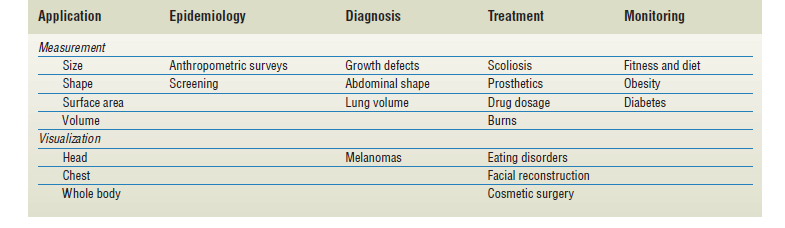
\includegraphics[width=15cm]{table1.png}
    \caption{3D Scanning Applications}\cite[]{treleaven_wells_2007}.
\end{table}

\section{Overview}
As mentioned before, project consists of developing a 3D scanner that is allowed to scan person and be able to use that data in order to be able to virtually fit different clothing.
This capstone project mainly focuses on the software and processing of the data for the 3D reconstruction.

The aim of this project is to develop algorithms and an implementation pipeline that will use the acquired image data as well as the reference pointcloud data in order to produce an accurate
and appropiately scaled 3D reconstructed model of a person.\\
This is reconstructed ans scaled model of the scanned person, is intended to be utilised as the model for testing virtual clothe fitting and be able to correctly determine the size of the garments. 
This technology could have a massive industry in the clothing industry and online retailers as this could solve an issue with the returns policy due to incorrect sizing for different customers groups.
\subsection{Methodology}
To achive the aim, a rig will be used to capture the data. The Rig will consist of a set of poles with multiple cameras. Furthermore a Lidar Intel RealSense L515 will be used to capture another image an the corresponding pointcloud that will be used for reference.
Once the rig captures the data (28 images) as well as the lidar data(1 image, 1 pointcloud), the images will be processed with photogrammetry approach with Meshroom. 
The Processed data from Meshroom will produce a preprocessed reconstruction mesh. 

After this the mesh will be processed in the developed algorithmic pipeline and it will be properly scaled with the reference pointcloud from the Lidar. 
Once the mesh has been processed and scaled, it will be reconstructed appropiatelyand it will generate a final model of the scanned person with the with only the necessary components and appropriate scale.

Once the process is completed the mesh will be saved to disk as a ply file that can be later use in other applications such as clothing fitting. 

\subsection{Structure}
This Report will start with a literature review in order to analyse and fully understand the algorithms and techniques that are used in both components. 
It will help to understand the techniques used in the photogrammetry step and the developed algorithm pipeline.

Following this, details will be presented and illustrated as to how the process is carried out and the results that were obtained from different data sets.
It will fully ilustrated how to import the data to Meshroom, what parameters are required to add and modify in order to change the most robust reconstruction. There will be an indetail explanation of what each step executes.

Furthermore, there will be an detailed explanation of the algorithm pipeline for data processing. Here it will be explain what each component is expected to execute as well as how it was created and wrapped into a framework.
\enlargethispage{\baselineskip}
\chapter{Literature Review}
Being able to scan different objects and subjects has been a challenging task for researchers. Getting an accurate spatial location of the objects is crucial for this type of application.
The use of 3D point clouds has facilitated this process as it allowed to obtain the following parameters:
\begin{itemize}[]
  \itemsep0em 
  \item Depth
  \item Intensity
  \item Pulse width
  \item Light echo
\end{itemize}
This information can be obtained with different kind of sensors. There is a wide variety of off the shelf sensors that can provide 3D point clouds. 
These sensors could either be stereo or multiview vision cameras, lasers, time-of-flight sensors (\textit{TOF}) and structured light sensors as stated by \Citet*{murcia_monroy_mora_2018}.

Many Scanning devices will use single or multiple of the above-mentioned sensors to acquire data. Once the data is obtained, it essential to have a framework for 3D data modelling and reconstruction.
The principle behind 3D data reconstruction is obtained with data fusion from RGB-D sensors. This kind of sensors provide 3 channels images RGB (red, green, blue) and the depth images are mapped to each pixel. Based on this data, 3D point clouds could be generated for data reconstruction.

Similarly many other scanning devices use photogrammetry as a technique in order to do the reconstruction. In this particular project Meshroom was used as a 3D photogrammetry reconstruction software.

Moreover, several open source libraries were used in order to process and scale the draft mesh. These open source libraries include PCL and Open3D. From these several algorithms were used that aid in the data processing and these will be explained below. 
\enlargethispage{\baselineskip}

\section{Photogrammetry}
Photogrammetry is decribed as the associated techniques with performing measurements of real-world objects and terrain features from images as mentioned by \Citet*{photogrammetry_def}.
Many of the applications include the quantification of distances, volumes,areas, heights, 3D topographic mapping, measuring of objects, extracion of 3D pointcloud for surfaces reconstruction as well as the generation of orthophotographs and digital elevation models.\Citep*{photogrammetry_def}.

In recent years, with the development of technologies pairing computer vision concepts \& algorithms and photogrammetry specifically \textit{Structure from Motion-Multiview Stereo (\textbf{SfM-MVS})}
has led to significant advances in 3D surface Reconstruction from images \Citep*{photogrammetry_def}.

The key principle behind all the photogrammetric measurements is associated with the mathematical \& geometrical reconstruction of the path of light rays from the object to the sensor camera in the exact moment of data image acquisition.
Thus, the fundamental concept of photogrammetry is the undertanding of geometric characteristics of a single photograph.

\begin{figure}[h]
  \centering
  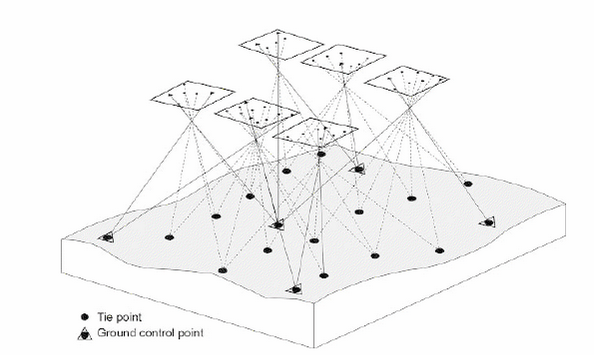
\includegraphics[width=0.8\textwidth]{photogrammetry.png}
  \caption{Photogrammetry Principle Illustration}\cite[]{photogrammetry_def}
  \label{fig:photogrammetry_principle} 
\end{figure}

\section{Meshroom}
Meshroom is a free, open-source 3D Reconstruction Software based on the AliceVision framework \Citep*{meshroom}.
AliceVision is a software framework based on photogrametric computer vision.  which focuses on the development of 3D Reconstruction and Camera Tracking Algorithms.
It aims to provide robust software foundation with novel computer vision algorithms that can be analysed, tested and reused.\\
Meshwoom was developed as collobaration project between industry and academia in order to develop cutting-edge algorithms that are robust and of high quality which are crucial for production environments.

\subsection*{Components Pipeline}
Meshroom can be downloaded and used in both Windows and Linux and it will require a powerfull CPU in order to have adequate performance. Also it will require an Nvidia GPU as it requires to run CUDA for different nodes and components.
Once meshroom is downloaded it can run in either platform. When it is executed the Meshroom GUI will appear and it will be similar to figure \ref{fig:meshroom_gui}

\begin{figure}[h]
  \centering
  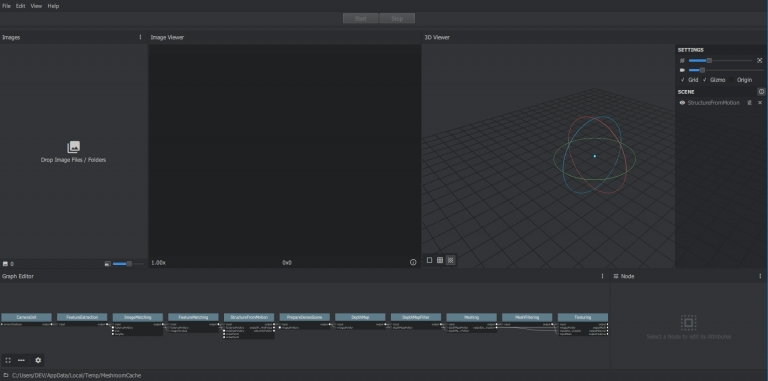
\includegraphics[width=1\textwidth]{meshroom_gui.jpg}
  \caption{Meshroom Graphical User Interface}\cite[]{meshroom}
  \label{fig:meshroom_gui} 
\end{figure}

\newpage
As mentioned before, meshroom is based on AliceVision's Framework. Therfore it follows a photogrametric pipeline for 3D reconstruction. 
This pipeline will have the following components:
\begin{itemize}
  \item Natural Feature Extraction
  \item Image Matching
  \item Features Matching
  \item Structure from Motion
  \item Depth maps estimation
  \item Meshing
  \item Texturing
  \item Localization
\end{itemize}

The pipeline will be included into Meshroom GUI and it will be used in the nodes. All the components in Meshroom will be embedded into different individual nodes that will be executed and produce individual results that will be send to the next node along in the pipeline.
As the nodes represent specific components of the reconstruction pipeline, these should be executed in a defined order.\\
The nodes in the defined order to reconstruct a 3D model from images include:
\begin{enumerate}
  \item Camera Initialization 
  \item Feature Extraction
  \item Image Matching
  \item Feature Matching
  \item Structure From Motion
  \item Prepare Dense Scene
  \item Depth Map
  \item Depth Map Filter
  \item Meshing
  \item Mesh Filtering
  \item Texturing
\end{enumerate}

\subsection{Camera Initialization}
Camera Initialization or \textit{"CameraInit"} loads the image metadata, sensor information, camera parameters and it will  generate viewpoints based on the images.
It is possible to use a mixture of cameras \& focal lengths. This node will generate a groups of intrinsics that are based on the images metadata, these grooup os intrinsics can be adjusted if the cameras have been fully calibrated.
The intrinsic include the camera matrix  which includes the focal length ($f_x$,$f_y$) and principal point ($x_0$,$y_0$).
\begin{equation*}
  Camera Intrinsics = 
  \begin{pmatrix}
  f_x & 0 & x_0 \\
  0 & f_y & y_0 \\
  0 & 0 & 1
  \end{pmatrix}
\end{equation*}
\label{equ:camera_intrisics}

The components in the node are described on table \ref{tab:CameraInit}
% Please add the following required packages to your document preamble:
% \usepackage{graphicx}
\begin{table}[h!]
  \centering
  \resizebox{\textwidth}{!}{%
  \begin{tabular}{|l|l|}
  \hline
  Viewpoints Input &
    \begin{tabular}[c]{@{}l@{}}viewpoints (1 Element for each loaded image) \\ - ID \\ - Pose ID \\ -  Image Path \\ - Intrinsic: Internal Camera Parameters (Intrinsic ID) \\ - Rig  (-1 - 200) \\ - Rig Sub-Pose: Rig Sub-Pose Parameters (-1 - 200)\\  - Image  Metadata: (list of metadata elements)\end{tabular} \\ \hline
  Intrinsic Camera Intrinsics &
    \begin{tabular}[c]{@{}l@{}}(1 Element for each loaded image) - ID - Initial Focal Length:  Initial Guess on the Focal Length \\ - Focal Length: Known/Calibrated Focal  Length \\ - Camera Type: pinhole’, ‘radial1’, ‘radial3’, ‘brown’,  ‘fisheye4’ \\ - \#Make: Camera Make (not included in this build, commented  out) \\ - \#Model: Camera Model \\ - \#Sensor Width: Camera Sensor Width \\ -  Width: Image - Width (0-10000) \\ - Height: Image Height (0-10000) - Serial  Number: Device Serial Number (camera and lens combined) \\ - Principal  Point: X (0-10000) Y(0-10000)\\ - DistortionParams: Distortion Parameters \\ -  Locked(True/False): If the camera has been calibrated, the internal  camera parameters (intrinsics) can be locked. It should improve  robustness and speedup the reconstruction.\end{tabular} \\ \hline
  Sensor Database &
    Camera sensor width database path \\ \hline
  Default Field Of View &
    Empirical value for the field of view in degree 45° (0°-180°) \\ \hline
  Verbose Level &
    verbosity level (fatal, error, warning, info, debug, trace) \\ \hline
  Output SfMData File &
    …/cameraInit.sfm \\ \hline
  \end{tabular}%
  }
  \caption{Meshroom CameraInit Node }
  \label{tab:CameraInit}
  \end{table}

\subsection{Feature Extraction}
% https://meshroom-manual.readthedocs.io/en/latest/feature-documentation/core/pipelines/photogrammetry.html
The key objective of this node is to extract distinctive pixel groups, which are to a certain extend invariant to a change in camera viewpoints during the image acquisition process.
Thus, a feature in this scene should have similar features descriptors in all the captures images.

One of the most used feature detection method is \textbf{SIFT} \textit{(Scale-invariant feature transform)} algorithm. 
The objective of SIFT is to extract discriminative patches in an initial image that later can be compared to discriminative patches of a second image, irrespective of scale, rotation and translation \Citep*{Lowe2004}.
As a relevant detail is only present at a specific scale, the extracted patches are centered around the point of interests. 
Therefore, the SIFT invarience can be used to deal with image transformations that occur when the viewpoints change during image acquisition.

Based on the representation of one image at different scales, SIFT is able to compute scale-space maxima of the Laplacian Representation. This is a defined image energy-based representation, using the differences of Gaussians.
This Maxima is associated to the points of interest in the image. 
Once this is processed, it samples for each of the this maxima a square image patch, whose origin is the maximum and "x" direction is the dominant gradient at the origin as suggested by \Citet*{Lowe2004} and\Citet*{Otero2014} .
For each keypoint, a description of these patches is associated. 

The description consists of statistics of gradients which is computed in regions around the keypoint. The size of the region is defined by the keypoint scale and the orientation by the dominant axis.
 It is also frequently stored in 128 bits.
 \enlargethispage{\baselineskip}

The number of extracted features could vary as a result of texture complexity, from one image to other ones or in different image sections. Hence, a post-filtering step controls the number of extrated features to a specified limit. 
Furthermore, grid filtering is used to ensure an even repartition in the image.

The components in the node are described on table \ref{tab:FeatureExtraction}

\begin{table}[h!]
  \centering
  \resizebox{\textwidth}{!}{%
  \begin{tabular}{|l|l|}
  \hline
  \multicolumn{1}{|c|}{Name} & Description                                                          \\ \hline
  Input                      & SfMData file.                                                        \\ \hline
  Describer Types &
    Describer types used to describe an image. ‘sift’, ‘sift*float’, ‘sift*upright’, ‘akaze’, ‘akaze*liop’, ‘akaze*mldb’, ‘cctag3’, ‘cctag4’, ‘sift*ocv’, ‘akaze*ocv’ \\ \hline
  Describer Preset &
    Control the ImageDescriber configuration (low, medium, normal, high, ultra). Configuration “ultra” can take long time ! \\ \hline
  Force CPU Extraction       & Use only CPU feature extraction.                                     \\ \hline
  Max Nb Threads &
    Specifies the maximum number of threads to run simultaneously (0 for automatic mode). (0-24) 0 \\ \hline
  Verbose Level              & verbosity level (fatal, error, warning, info, debug, trace).         \\ \hline
  Output Folder              & Output path for the features and descriptors files (*.feat, *.desc). \\ \hline
  \end{tabular}%
  }
  \caption{Meshroom FeatureExtraction Node Settings}
  \label{tab:FeatureExtraction}
  \end{table}

  
\subsection{Image Matching}
The principle behind this node is to find images that point to the same areas of interest. Therefore, image retrieval techniques are implemented with the purpose of finding images 
that share content without the demand of resolving all the  detailed feature matches. Hence, the goal is to simplify the image in a compact image descriptor. This allows to efficiencly compute the distance between all images descriptors.

A vocabulary tree is one of the widely used methodologies to generate the image descriptor. It works by passing all the extracted features descriptors into it. Then it performs a classification process, which compares their descriptors to the ones on each node of the vocabulary tree as mentioned by \Citet*{Nister2006}.
Each feature descriptor is associated with one leaf, which can be stored with an standard index (\textit{The index of this leaf in the tree}).Thus, the collection of leaves indices represents the image descriptor \Citep*{Nister2006}.

The components in the node are described on table \ref{tab:ImageMatching}

\begin{table}[h!]
  \centering
  \resizebox{\textwidth}{!}{%
  \begin{tabular}{|l|l|}
  \hline
  \multicolumn{1}{|c|}{\textbf{Name}} & \multicolumn{1}{c|}{\textbf{Description}}                               \\ \hline
  Image                               & SfMData file                                                            \\ \hline
  Features Folders                    & Folder(s) containing the extracted features and descriptors             \\ \hline
  Tree                                & Input name for the vocabulary tree file ALICEVISION\_VOCTREE            \\ \hline
  Weights &
    Input name for the weight file, if not provided the weights will be computed on the database built with the provided set \\ \hline
  Minimal Number of Images &
    \begin{tabular}[c]{@{}l@{}}Minimal number of images to use the vocabulary tree. \\ If we have  less features than this threshold, we will compute all matching  combinations\end{tabular} \\ \hline
  Max Descriptors                     & Limit the number of descriptors you load per image. Zero means no limit \\ \hline
  Nb Matches &
    The number of matches to retrieve for each image (If 0 it will retrieve all the matches) 50 (0-1000) \\ \hline
  Verbose Level                       & verbosity level (fatal, error, warning, info, debug, trace)             \\ \hline
  Output List File                    & Filepath to the output file with the list of selected image pairs       \\ \hline
  \end{tabular}%
  }
  \caption{Meshroom Image Matching Node}
  \label{tab:ImageMatching}
  \end{table}



\subsection{Feature Matching}
The key component of feature matching node is to be able to match all features between potential image pairs.
Initially, the node performs a photometric process that creates matches between the descriptors from 2 separe images. For each feature in image "A", a list of potential features in image "B" is generated.
The descriptor space is not linear and defined space, which causes uncertainty in the validity of the matches due to the absolute distance values. 
Furthermore, in order to remove bad candidates, an assumption process associates only one valid match in the other image.
Hence, for each feature descriptor on Image "A", two of the closests descriptors in the image are used with a relative threshold between them which provides a robust criteria as mentioned by \Citet*{Lowe2004}.

This process will provide a photometric list of feature matching candidates. Afterwards, the images features positions are used in a geometrica
filtering process that uses epipolar geometry in an outlier detection framework, which is RANSAC (\textit{"Random Sample Consensus"}).
Moreover, a random selection process uses a small set of feature correspondances and it computers either the fundamental or essential matrix. 
Once this process is completed, the number of features verifies and validates this model and iterates through the RANSAC framework \Citep*{FLANN2009}.
\enlargethispage{\baselineskip}
The components in the node are described on table \ref{tab:FeatureMatching}

\begin{table}[h!]
  \centering
  \resizebox{\textwidth}{!}{%
  \begin{tabular}{|l|l|}
  \hline
  \multicolumn{1}{|c|}{\textbf{Name}} &
    \multicolumn{1}{c|}{\textbf{Description}} \\ \hline
  Input &
    SfMData file \\ \hline
  Features Folder &
     \\ \hline
  Features Folders &
    Folder(s) containing the extracted features and descriptors \\ \hline
  Image Pairs List &
    Path to a file which contains the list of image pairs to match \\ \hline
  Describer Types &
    Describer types used to describe an image **sift**'/ 'sift\_float'/ 'sift\_upright'/ 'akaze'/ 'akaze\_liop'/ 'akaze\_mldb'/ 'cctag3'/ 'cctag4'/ 'sift\_ocv'/ 'akaze\_ocv \\ \hline
  Photometric Matching Method &
    \begin{tabular}[c]{@{}l@{}}For Scalar based regions descriptor \\ * BRUTE\_FORCE\_L2: L2  BruteForce matching\\ * ANN\_L2: L2 Approximate Nearest Neighbor  matching \\ * CASCADE\_HASHING\_L2: L2 Cascade Hashing matching\\ *  FAST\_CASCADE\_HASHING\_L2: L2 Cascade Hashing with precomputed hashed  regions (faster than CASCADE\_HASHING\_L2 but use more memory) \\ For Binary  based descriptor  \\ * BRUTE\_FORCE\_HAMMING: BruteForce Hamming matching\end{tabular} \\ \hline
  Geometric Estimator &
    Geometric estimator: (acransac:  A-Contrario Ransac //  loransac: LO-Ransac (only available for fundamental\_matrix model) \\ \hline
  Geometric Filter Type &
    Geometric validation method to filter features matches: **fundamental\_matrix** // essential\_matrix // homography\_matrix /// homography\_growing // no\_filtering' \\ \hline
  Distance Ratio &
    Distance ratio to discard non meaningful matches 0.8 (0.0 - 1) \\ \hline
  Max Iteration &
    Maximum number of iterations allowed in ransac step 2048 (1 - 20000) \\ \hline
  Max Matches &
    Maximum number of matches to keep (0 - 10000) \\ \hline
  Save Putative Matches &
    putative matches (True/False) \\ \hline
  Guided Matching &
    the found model to improve the pairwise correspondences (True/False) \\ \hline
  Export Debug Files &
    debug files (svg/ dot) (True/False) \\ \hline
  Verbose Level &
    verbosity level (fatal, error, warning, info, debug, trace) \\ \hline
  Output Folder &
    Path to a folder in which computed matches will be stored \\ \hline
  \end{tabular}%
  }
  \caption{Meshroom Feature Matching Node}
  \label{tab:FeatureMatching}
  \end{table}

\newpage
\subsection{Structure From Motion}

The Structure From Motion Node carries out the 3D points reconstruction freom the input images. The key behind this node is to be able to comprenhend
the geometric relationship behind all the views from the input images, and decifer the rigid scene structure (3D PointCloud) along with the pose (position \& orientation) and internal calibration of the cameras as mentioned by \Citet*{Cheng2014}
This is an incremental process pipeline which associated with a growing reconstruction process. It  initially computes an starting two-view point reconstruction which is iteratively extended by adding new views \Citep*{Cheng2014}.

It starts by fusing all feature matches between all images and store them in tracks. Each track represents a point in space, which is visible from multiple cameras. 
Nevertheless, at this stage of the pipeline, many outliers are present,therefore during matches fusion, incorrect tracks are removed \citep*{Fischler1981RandomSC}.

Afterwards, the incremental algorithm chooses the best initial image pair. This choice is very important for the quality of the final reconstruction, hence it should provide robust matches and reliable geometric information as suggested by \citet*{Moulon2012}.
Therefore, this image pair maximises the number of matches and the repartition of features correspondances in all images. On the other hand, the angle between the cameras must be able to provide with reliable gemoetric information.
Then, it computes the fundamental matrix between these two images considering the first image as the origin of the coordinate system \Citep*{Kneip2011}. As the pose of the first two cameras is known, 
it is possible to triangulate the matching 2D features into 3D points. 

Once this step finishes, the \textit{Next Best Views Selection} algorithm selects all the images that have enough number of associations with the 3D reconstructed features.
Based on 2D-3D associations, it performs the resectioning of each of the new cameras \citep*{Lepetit2008EPnPAA}. The resectioning is a \textbf{Perspective-n-Point} algorithm (\textbf{\textit{PnP}}) in a
\textbf{RANSAC} framework that finds the pose of the camera that validates the features association. Similarity, a non-linear minimization proceess is performed on each camera, to refine the end pose \citep*{Nister2004}.

From these new camera poses, some tracks become visible by two or more resected cameras and it triangulates them. A Bundle Adjustment process starts and refines everything such as:
intrinsic and extrinsic parameters of all cameras, as well as the position of all 3D points as suggested by \citet*{Shah2014}. A filter processes the result of the Bundle Adjustment process and removes all osbservations that have a high reprojection error or not enough angles between viewpoints.

In the new points tringulation process, it uses more image candidates for the best views selection. It iterates by adding cameras and tringulatins new 2D features into 3D points and removes 3D points that become invalid in the process,until no more new views can be localized \citep*{Shah2014}.

The components in the node are described on table \ref{tab:StructureFromMotion}

\begin{table}[h!]
  \centering
  \resizebox{\textwidth}{!}{%
  \begin{tabular}{|l|l|}
  \hline
  \textbf{Input}                      & \textbf{SfMData file}                                                                              \\ \hline
  Features Folder                     & Folder(s) containing the extracted features and descriptors.                                       \\ \hline
  Matches Folders                     & Folder(s) in which computed matches are stored.                                                    \\ \hline
  Describer Types &
    Describer types used to describe an image. ‘sift’, ‘sift*float’, ‘sift*upright’, ‘akaze’, ‘akaze*liop’, ‘akaze*mldb’, ‘cctag3’, ‘cctag4’, **’siftocv’, ‘akazeocv’ \\ \hline
  Localizer Estimator                 & Estimator type used to localize cameras (acransac, ransac, lsmeds, loransac, maxconsensus).        \\ \hline
  Observation Constraint &
    \begin{tabular}[c]{@{}l@{}}Observation constraint mode used in the optimization: \\ Basic:  Use standard reprojection error in pixel coordinates, \\ Scale: Use  reprojection error in pixel coordinates but relative to the feature  scale\end{tabular} \\ \hline
  Localizer Max Ransac Iterations     & Maximum number of iterations allowed in ransac step. (1-20000) 4096                                \\ \hline
  Localizer Max Ransac Error &
    \begin{tabular}[c]{@{}l@{}}Maximum error (in pixels) allowed for camera localization  (resectioning).\\ If set to 0, it will select a threshold according to the  localizer estimator used (if ACRansac, it will analyze the input data  to select the optimal value). (0.0-100-0) 0.0\end{tabular} \\ \hline
  Lock Scene Previously Reconstructed & This option is useful for SfM augmentation. Lock previously reconstructed poses and intrinsics.    \\ \hline
  Local Bundle Adjustment &
    It reduces the reconstruction time, especially for large datasets  (500+ images) by avoiding computation of the Bundle Adjustment on areas  that are not changing. \\ \hline
  LocalBA Graph Distance              & Graph-distance limit to define the Active region in the Local Bundle Adjustment strategy. (2-10) 1 \\ \hline
  Maximum Number of Matches &
    \begin{tabular}[c]{@{}l@{}}Maximum number of matches per image pair (and per feature type).\\  This can be useful to have a quick reconstruction overview. 0 means no  limit. (0-50000) 1\end{tabular} \\ \hline
  Minimum Number of Matches &
    \begin{tabular}[c]{@{}l@{}}Minimum number of matches per image pair (and per feature type). \\ This can be useful to have a meaningful reconstruction with accurate  keypoints. 0 means no limit. (0-50000) 1\end{tabular} \\ \hline
  Min Input Track Length              & Minimum track length in input of SfM (2-10)                                                        \\ \hline
  Min Observation For Triangulation &
    \begin{tabular}[c]{@{}l@{}}Minimum number of observations to triangulate a point. \\ Set it to 3  (or more) reduces drastically the noise in the point cloud, but the  number of final poses is a little bit reduced (from 1.5\% to 11\% on the  tested datasets). (2-10)\end{tabular} \\ \hline
  Min Angle For Triangulation         & Minimum angle for triangulation. (0.1-10) 3.0                                                      \\ \hline
  Min Angle For Landmark              & Minimum angle for landmark. (0.1-10) 2.0                                                           \\ \hline
  Max Reprojection Error              & Maximum reprojection error. (0.1-10) 4.0                                                           \\ \hline
  Min Angle Initial Pair              & Minimum angle for the initial pair. (0.1-10) 5.0                                                   \\ \hline
  Max Angle Initial Pair              & Maximum angle for the initial pair. (0.1-60) 40.0                                                  \\ \hline
  Use Only Matches From Input Folder &
    Use only matches from the input matchesFolder parameter. Matches folders previously added to the SfMData file will be ignored. \\ \hline
  Use Rig Constraint                  & Enable/Disable rig constraint.                                                                     \\ \hline
  Force Lock of All Intrinsic Camera Parameters. &
    \begin{tabular}[c]{@{}l@{}}Force to keep constant all the intrinsics parameters of the  cameras (focal length, principal point, distortion if any) during the  reconstruction. \\ This may be helpful if the input cameras are already  fully calibrated.\end{tabular} \\ \hline
  Filter Track Forks &
    \begin{tabular}[c]{@{}l@{}}Enable/Disable the track forks removal. \\ A track contains a fork  when incoherent matches lead to multiple features in the same image for a  single track.\end{tabular} \\ \hline
  Initial Pair A                      & Filename of the first image (without path).                                                        \\ \hline
  Initial Pair B                      & Filename of the second image (without path).                                                       \\ \hline
  Inter File Extension                & Extension of the intermediate file export. (‘.abc’, ‘.ply’)                                        \\ \hline
  Verbose Level                       & Verbosity level (fatal, error, warning, info, debug, trace).                                       \\ \hline
  Output SfMData File                 & Path to the output sfmdata file (sfm.abc)                                                          \\ \hline
  Output SfMData File                 & Path to the output sfmdata file with cameras (views and poses). (cameras.sfm)                      \\ \hline
  Output Folder                       & Folder for intermediate reconstruction files and additional reconstruction information files.      \\ \hline
  \end{tabular}%
  }
  \caption{Meshroom StructureFromMotion Node}
  \label{tab:StructureFromMotion}
  \end{table}


\newpage
\subsection{Prepare Dense Scene}
This node undistorts the images and it genera etes EXR images.
The components in the node are described on table \ref{tab:PrepareDenseScene}

\begin{table}[h!]
  \centering
  \resizebox{\textwidth}{!}{%
  \begin{tabular}{|l|l|}
  \hline
  \multicolumn{1}{|c|}{\textbf{Name}} & \multicolumn{1}{c|}{\textbf{Description}}                         \\ \hline
  Input                               & SfMData file                                                      \\ \hline
  ImagesFolders & Use images from specific folder(s). Filename should be the same or the image uid.      \\ \hline
  Output File Type                    & Output file type for the undistorted images. (jpg, png, tif, exr) \\ \hline
  Save Metadata & Save projections and intrinsics information in images metadata (only for .exr images). \\ \hline
  Save Matrices Text Files            & Save projections and intrinsics information in text files.        \\ \hline
  Correct images exposure             & Apply a correction on images Exposure Value                       \\ \hline
  Verbose Level                       & {[}‘fatal’, ‘error’, ‘warning’, ‘info’, ‘debug’, ‘trace’{]}       \\ \hline
  Output                              & MVS Configuration file (desc.Node.internalFolder + ‘mvs.ini)      \\ \hline
  Undistorted images                  & List of undistorted images.                                       \\ \hline
  \end{tabular}%
  }
  \caption{Meshroom Prepare Dense Scene Node}
  \label{tab:PrepareDenseScene}
  \end{table}


\subsection{Depth Map}

This step in the pipeline retrieves the depth value of each pixel for all cameras that were processes by the StructureFromMotion Node.
It uses Semi-Global Matching method as proposed by \citet*{Hirschmuller2005}.

For each image, it selects the \textbf{"N"} best \& closests cameras around. It chooses fronto-parallel planes based on the intersection of the optical axis with the pixels of the choosen neighboring cameras \Citep*{Hirschmuller2005}.
This produces a volume \textbf{W,H,Z} with several depth candidates per pixel and it estimates the similarity for all of these. The Similarity is calculated by the \textit{Zero Mean Normalized Cross-Correlation (ZNCC)}
of a small patch in the principal image which is reprojected into at the other camera, which creates a volume of similarities as suggested by \Citet*{Strecha2006}.
For each neighboring image, it accumulates similarities in this volume. Nevertheless, this volume is noisy,therefore,  there is a filter in each step along X \& Y axis which reduces the isolated high values.
Finally, it selects the local minima and replaces the selected plane index with a depth value stored into a depth map \Citep*{Scharstein2002}. This depth map has banding artifacts as it based on the original selection of depth values as mentioned by \Citet*{Scharstein2002}.
Thus, a refinement process calculates the depth values with sub-pixel accuracy.

The components in the node are described on table \ref{tab:DepthMap}

\begin{table}[h!]
  \centering
  \resizebox{\textwidth}{!}{%
  \begin{tabular}{|l|l|}
  \hline
  \multicolumn{1}{|c|}{\textbf{Name}} & \multicolumn{1}{c|}{\textbf{Description}}                               \\ \hline
  MVS Configuration File:             & SfMData file.                                                           \\ \hline
  Images Folder                  & Use images from a specific folder instead of those specify in the SfMData file. Filename should be the image uid. \\ \hline
  Downscale                           & Image downscale factor (1, 2, 4, 8, 16)                                 \\ \hline
  Min View Angle                      & Minimum angle between two views.(0.0 - 10.0)                            \\ \hline
  Max View Angle                      & Maximum angle between two views. (10.0 - 120.0)                         \\ \hline
  SGM: Nb Neighbour Cameras           & Semi Global Matching: Number of neighbour cameras (1 - 100)             \\ \hline
  SGM: WSH: Semi Global Matching & Half-size of the patch used to compute the similarity (1 - 20)                                                    \\ \hline
  SGM: GammaC                         & Semi Global Matching: GammaC Threshold (0 - 30)                         \\ \hline
  SGM: GammaP                         & Semi Global Matching: GammaP Threshold (0 - 30)                         \\ \hline
  Refine: Number of samples           & (1 - 500)                                                               \\ \hline
  Refine: Number of Depths            & (1 - 100)                                                               \\ \hline
  Refine: Number of Iterations        & (1 - 500)                                                               \\ \hline
  Refine: Nb Neighbour Cameras        & Refine: Number of neighbour cameras. (1 - 20)                           \\ \hline
  Refine: WSH                         & Refine: Half-size of the patch used to compute the similarity. (1 - 20) \\ \hline
  Refine: Sigma                       & Refine: Sigma Threshold (0 - 30)                                        \\ \hline
  Refine: GammaC                      & Refine: GammaC Threshold. (0 - 30)                                      \\ \hline
  Refine: GammaP                      & Refine: GammaP threshold. (0 - 30)                                      \\ \hline
  Refine: Tc or Rc pixel size    & Use minimum pixel size of neighbour cameras (Tc) or current camera pixel size (Rc)                                \\ \hline
  Verbose Level                       & verbosity level (fatal, error, warning, info, debug, trace)             \\ \hline
  Output                              & Output folder for generated depth maps                                  \\ \hline
  \end{tabular}%
  }
  \caption{Meshroom Depth MapNode}
  \label{tab:DepthMap}
  \end{table}
% https://meshroom-manual.readthedocs.io/en/latest/feature-documentation/core/pipelines/photogrammetry.html

\newpage
\subsection{Depth Map Filter}
This node is in charge of processing the DepthMap Node results s the original depth maps will not be entirely consistent.
Certain depth maps will interprete to see areas that are occluded by other dept maps. Thus, this step of the pipeline isolates these areas and ensures depth consistency.

The components in the node are described on table \ref{tab:DepthMapFilter}

\begin{table}[h!]
  \centering
  \resizebox{\textwidth}{!}{%
  \begin{tabular}{|l|l|}
  \hline
  \multicolumn{1}{|c|}{\textbf{Name}}     & \multicolumn{1}{c|}{\textbf{Description}}                   \\ \hline
  Input                                   & SfMData file                                                \\ \hline
  Depth Map Folder                        & Input depth map folder                                      \\ \hline
  Number of Nearest Cameras               & Number of nearest cameras used for filtering 10 (0 - 20)    \\ \hline
  Min Consistent Cameras                  & Min Number of Consistent Cameras 3 (0 - 10)                 \\ \hline
  Min Consistent Cameras Bad Similarity & Min Number of Consistent Cameras for pixels with weak similarity value 4 (0 - 10) \\ \hline
  Filtering Size in Pixels                & Filtering size in Pixels (0 - 10)                           \\ \hline
  Filtering Size in Pixels Bad Similarity & Filtering size in pixels (0 - 10)                           \\ \hline
  Verbose Level                           & verbosity level (fatal, error, warning, info, debug, trace) \\ \hline
  Output                                  & Output folder for generated depth maps                      \\ \hline
  \end{tabular}%
  }
  \caption{Meshroom Depth Map Filter Node}
  \label{tab:DepthMapFilter}
  \end{table}



\subsection{Meshing}
The main purpose of this node is to construct a dense geometric surface representation of the scene.
Initially, it fuses all the processed depth maps into a global octree and where it is compatible it will merge depth values into the octree cells.
Afterwards, the node performs a 3D Delaunay tetrahedralization process. Subsequenly, a complex voting procedure computes the weighs on cells and weights the faces connecting 
the cells \citep*{Jancosek2011}  as mentioned by  \Citet*{Jancosek2014}.

A Graph Cut Max-Flow \Citep*{Boykov2004} is applied to efficiencly reduce the volume, which represents the extrated mesh surface. 
Furthermore, it filters bad cells on the surface and applies a Laplacian filtering process on the Mesh to remove local artifacts.

The components in the node are described on table \ref{tab:Meshing}

\begin{table}[h!]
  \centering
  \resizebox{\textwidth}{!}{%
  \begin{tabular}{|l|l|}
  \hline
  \multicolumn{1}{|c|}{\textbf{Name}}       & \multicolumn{1}{c|}{\textbf{Description}}                                                \\ \hline
  Input                                     & SfMData file.                                                                            \\ \hline
  Depth Maps Folder                         & Input depth maps folder                                                                  \\ \hline
  Filtered Depth Maps Folder                & Input filtered depth maps folder                                                         \\ \hline
  Estimate Space From SfM                   & Estimate the 3d space from the SfM                                                       \\ \hline
  Min Observations For SfM Space Estimation & Minimum number of observations for SfM space estimation. (0-100) 3                       \\ \hline
  Min Observations Angle For SfM Space Estimation &
    Minimum angle between two observations for SfM space estimation. (0-120) 10 \\ \hline
  Max Input Points                          & Max input points loaded from depth map images (500**000** - 500000000)                   \\ \hline
  Max Points                                & Max points at the end of the depth maps fusion (100**000** - 10000000)                   \\ \hline
  Max Points Per Voxel                      & (500**000** – 30000000)                                                                  \\ \hline
  Min Step &
    \begin{tabular}[c]{@{}l@{}}The step used to load depth values from depth maps is computed  from maxInputPts. \\ Here we define the minimal value for this step, so on  small datasets we will not spend too much time at the beginning loading  all depth values (1- 20) 2\end{tabular} \\ \hline
  Partitioning                              & (singleBlock, auto)                                                                      \\ \hline
  Repartition                               & (multiResolution, regularGrid)                                                           \\ \hline
  angleFactor                               & (0.0-200.0) 15.0                                                                         \\ \hline
  simFactor                                 & (0.0-200.0) 1.0                                                                          \\ \hline
  pixSizeMarginInitCoef                     & (0.0-10.0) 2.0                                                                           \\ \hline
  pixSizeMarginFinalCoef                    & (0.0-10.0) 4.0                                                                           \\ \hline
  voteMarginFactor                          & (0.1-10.0) 4.0                                                                           \\ \hline
  contributeMarginFactor                    & (0.0-10.0) 2.0                                                                           \\ \hline
  simGaussianSizeInit                       & (0.0-50) 10.0                                                                            \\ \hline
  simGaussianSize                           & (0.0-50) 0.1                                                                             \\ \hline
  minAngleThreshold                         & (0.0-10.0) 0.01                                                                          \\ \hline
  Refine Fuse                               & Refine depth map fusion with the new pixels size defined by angle and similarity scores. \\ \hline
  Add Landmarks To The Dense Point Cloud    & Add SfM Landmarks to the dense point cloud.                                              \\ \hline
  Colorize Output                           & Whether to colorize output dense point cloud and mesh.                                   \\ \hline
  Save Raw Dense Point Cloud                & Save dense point cloud before cut and filtering.                                         \\ \hline
  Verbose Level                             & verbosity level (fatal, error, warning, info, debug, trace).                             \\ \hline
  Output Mesh                               & Output mesh (OBJ file format). mesh.obj                                                  \\ \hline
  Output Dense Point Cloud                  & Output dense point cloud with visibilities (SfMData file format). densePointCloud.abc    \\ \hline
  \end{tabular}%
  }
  \caption{Meshroom Meshing Node}
  \label{tab:Meshing}
  \end{table}

\subsection{Mesh Filtering}

This node filters and removes the unwanted elements from the resulting mesh.
The components in the node are described on table \ref{tab:MeshFiltering}

\begin{table}[h!]
  \centering
  \resizebox{\textwidth}{!}{%
  \begin{tabular}{|l|l|}
  \hline
  \multicolumn{1}{|c|}{\textbf{Name}} & \multicolumn{1}{c|}{\textbf{Description}}                    \\ \hline
  Input                               & Input Mesh (OBJ file format)                                 \\ \hline
  Filter Large Triangles Factor &
    \begin{tabular}[c]{@{}l@{}}Remove all large triangles. We consider a triangle as large if  one edge is bigger than N times the average edge length. \\ Put zero to  disable it. 60 (1 - 100)\end{tabular} \\ \hline
  Keep Only the Largest Mesh          & Keep only the largest connected triangles group (True/False) \\ \hline
  Nb Iterations                       & 5 (0 - 50)                                                   \\ \hline
  Lambda                              & 1 (0-10                                                      \\ \hline
  Verbose Level                       &                                                              \\ \hline
  Verbose Level                       & {[}‘fatal’, ‘error’, ‘warning’, ‘info’, ‘debug’, ‘trace’{]}  \\ \hline
  Output mesh                         & Output mesh (OBJ file format) internalFolder + ‘mesh.obj     \\ \hline
  \end{tabular}%
  }
  \caption{Meshroom Mesh FilteringNode}
  \label{tab:MeshFiltering}
  \end{table}

\subsection{Texturing}
The principle of this components is to create a texture of the generated mesh.
If the mesh has no correspondent UV, it computes auomatic UV maps. It uses basic UV mapping approach to reduced the texture space as proposed by \Citet*{Levy2002}.

For each triangle, it uses the visibility information associated to each vertex in order to, retrieve texture candidates.
It filters the cameras that do not have a good angle to the surface to favourable fronto-parallel cameras to average the pixel values.
Furthermore, it uses a generalization of multiband blending as described by \Citet*{Burt1983AMS}. Thus, it averages more views in the low frequencies in comparison to the high frequencies.

The components in the node are described on table \ref{tab:Texturing}

\begin{table}[h!]
  \centering
  \resizebox{\textwidth}{!}{%
  \begin{tabular}{|l|l|}
  \hline
  \textbf{MVS Configuration file} & \textbf{…/mvs.ini}                                                                             \\ \hline
  Input Dense Reconstruction      & Path to the dense reconstruction result (mesh with per vertex visibility)                      \\ \hline
  Other Input Mesh                & Optional input mesh to texture. By default, it will texture the result of the reconstruction.  \\ \hline
  Texture Side                    & Output texture size 1024, 2048, 4096, 8192, 16384                                              \\ \hline
  Texture Downscale               & Texture downscale factor1, 2, 4, 8                                                             \\ \hline
  Texture File Type               & Texture File Type ‘jpg’, ‘png’, ‘tiff’, ‘exr’                                                  \\ \hline
  Unwrap Method &
    \begin{tabular}[c]{@{}l@{}}Method to unwrap input mesh if it does not have UV coordinates Basic  (\textgreater 600k faces) fast and simple. \\ Can generate multiple atlases LSCM  (\textless{}= 600k faces): optimize space. Generates one atlas ABF (\textless{}= 300k  faces): optimize space and stretch. \\ Generates one atlas\end{tabular} \\ \hline
  Fill Holes                      & Fill Texture holes with plausible values True/False                                            \\ \hline
  Padding                         & Texture edge padding size in pixel (0-100)                                                     \\ \hline
  Max Nb of Images For Fusion     & Max number of images to combine to create the final texture (0-10)                             \\ \hline
  Best Score Threshold            & 0.0 to disable filtering based on threshold to relative best score (0.0-1.0)                   \\ \hline
  Angle Hard Threshold            & 0.0 to disable angle hard threshold filtering (0.0, 180.0)                                     \\ \hline
  Force Visible By All Vertices   & Triangle visibility is based on the union of vertices visiblity.True/False                     \\ \hline
  Flip Normals &
    Option to flip face normals. It can be needed as it depends on  the vertices order in triangles and the convention change from one  software to another. \\ \hline
  Visibility Remapping Method     & Method to remap visibilities from the reconstruction to the input mesh (Pull, Push, PullPush). \\ \hline
  Verbose Level                   & verbosity level (fatal, error, warning, info, debug, trace).                                   \\ \hline
  Output Folder                   & Folder for output mesh: OBJ, material and texture files.                                       \\ \hline
  Output Mesh                     & Folder for output mesh: OBJ, material and texture files. internalFolder + ‘texturedMesh.obj    \\ \hline
  Output Material                 & Folder for output mesh: OBJ, material and texture files. internalFolder + ‘texturedMesh.mtl    \\ \hline
  Output Textures                 & Folder for output mesh: OBJ, material and texture files. internalFolder + ‘texture\_*.png      \\ \hline
  \end{tabular}%
  }
  \caption{Meshroom Texturing Node}
  \label{tab:Texturing}
  \end{table}


\section{PCL}
The \textbf{Point Cloud Library (PCL)} is a large scale, open project used for point cloud processing.\
The PCL framework contains multiple state-of-the art algorithms ranging from feature estimation,registration,filtering, model fitting to segmentation \Citep*{Rusu_ICRA2011_PCL}. 
PCL is a cross platform library and it is compatible with Windows, Linux and macOS.

The PCL framework is divided into a series of modular libraries such as:
\begin{multicols}{2}
\begin{itemize}
  \item Filters
  \item Features
  \item Keypoints
  \item Kegistration
  \item kdtree
  \item octree
  \item Segmentation
  \item Sample Consensus
  \item Surface
  \item Recognition
  \item IO 
  \item Visualization
\end{itemize}
\end{multicols}

These series of modular libraries  have a series of embedded algorithms  that can be used in scenarios such as: filtering outliers from noisy data, stitch multiple 3D pointclouds,
segment relevants parts of the scene \& point cloud, extract keypoints and compute image descriptors to be able to recognize real world objects based on geometric appearence, among many other possible implementations.

The selected components and algorithms that were used in this project include: 

\begin{itemize}
  \item Statistical Outlier Removal Filter
  \item Pass Through Filter
  \item Voxel Grid Filtering
  \item Plane Model Segmentation
  \item KdTree
  \item Euclidean Cluster Extraction
  \item Principal Component Analysis
  \item Moving Least Squares
  \item Poisson Surface Reconstruction 
\end{itemize}
%https://pcl.readthedocs.io/projects/tutorials/en/latest/index.html#i-o


\subsection{Statistical Outlier Removal Filter}
% https://pcl.readthedocs.io/projects/tutorials/en/latest/statistical_outlier.html#statistical-outlier-removal
%https://pcl.readthedocs.io/projects/tutorials/en/latest/statistical_outlier.html#statistical-outlier-removal

This component of the PCL library aims to remove noisy measurements (outliers) from a point cloud dataset using statistical analysis techniques \Citep*{Rusu_ICRA2011_PCL}.

Typically, Laser Scans produces point cloud datasets with various point densities.Similarly, measurement errors generate sparse outliers that can corrupt the results of the dataset.
This, complicates process of estimating local point cloud characteristics in particular surface normals and curvature changes. Hence, leading to erroneous values, that can create failures in the point cloud registration process.
Some of these irregularities in the dataset, can be addressed with a statistical analysis performed on each point's neighborhood, and removing the points that do not meet a specified criteria as mentioned by \Citet*{Rusu_ICRA2011_PCL}.
The sparse outlier removal is built on  the computation of the distribution  of point to neightbors distances of the source dataset \Citep*{Rusu_ICRA2011_PCL}.
For each point, it computes the mean distance from the points to all the corresponding neighbors. This process assumes that the resulting distribution is Gaussian with a standard deviation and a mean.
Then all points whose mean distances are outside an interval defined by global distances (mean \& standard deviation) can be expressed as an outlier and it can be removed from the dataset as suggested by \Citet*{Rusu_ICRA2011_PCL}.

Figure \ref{fig:statistical_removal_2} illustrates the results of the sparce outlier analysis and  removal process.
The initial dataset is on the left and the processed result in on the right. Furthermore, the graph on the right, illustrates the mean k-nearest neighbour distances in a point 
neighborhood, before and after the filtering process \cite[]{Rusu_ICRA2011_PCL}.

\begin{figure}[H]%this figure will be at the right
  \centering
  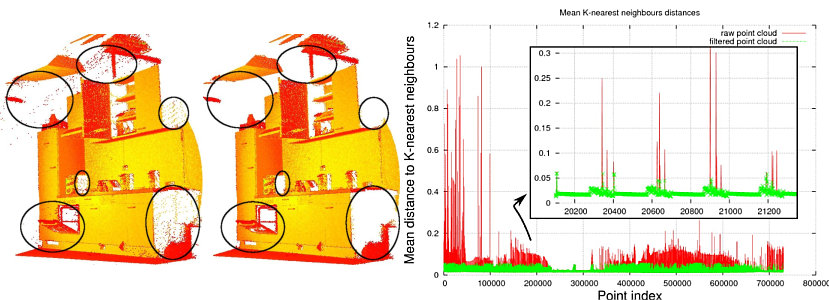
\includegraphics[width=1\textwidth]{statistical_removal_2.jpg}
 \caption{Removing outliers using a StatisticalOutlierRemoval filter}\cite[]{Rusu_ICRA2011_PCL}
 \label{fig:statistical_removal_2} 
\end{figure}

\subsection{Pass Through Filter}
%https://pcl.readthedocs.io/projects/tutorials/en/latest/passthrough.html#passthrough
This component of the PCL library has embedded two main components of the framework. 
The \textbf{PassThrough} components uses the base \textbf{Filter} class methods to pass through all the data that satisfies certain contrains.

PassThrough passes points in a pointcloud based on constrains for one specific field of the point type \Citep*{Rusu_ICRA2011_PCL}.
It iterates through the entire input pointcloud once, and automatically filters non-finite points, including the points outside the interval specfied by \textit{setFilterLimits()}, 
that only applies uniquely to the configured field \textit{setFilterFieldName()}. 
The component \textit{setFilterLimits()} sets the numerical limits for the field for data filtering, whereas \textit{setFilterFieldName()} configures the name of the field that will be used for data filtering.

Therefore, this component performs a filter along a given dimension, which essentially removes the values that are either outside or inside the configured range.
The image \ref{fig:pass_through} illustrates the process. The pointcloud has five points, after filtering the green points represents the remaining end result and the red points are the points that were removed by the filter.


\begin{figure}[H]%this figure will be at the right
  \centering
  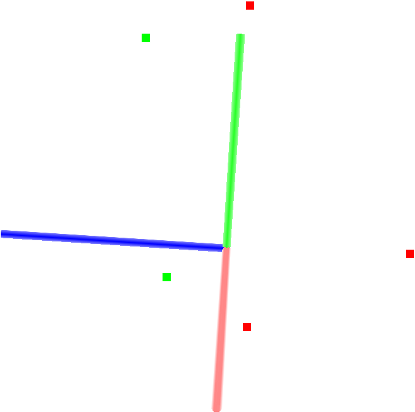
\includegraphics[width=0.4\textwidth]{passthrough_2.png}
 \caption{Filtering a PointCloud using a PassThrough filter}\cite[]{Rusu_ICRA2011_PCL}
 \label{fig:pass_through} 
\end{figure}

\subsection{Voxel Grid Filtering}
%https://pcl.readthedocs.io/projects/tutorials/en/latest/voxel_grid.html#voxelgrid

A voxel Grid illustraters a value on a regular grid in 3D space. A Voxel is an image of 3D space region  which is limited by defined sizes, which has its corresponding nodal point coordinates in an accepted system,
own form, owm state parameter that demostraters it belongs to some modelled object and it associated properties of the modelled region \Citep*{SHCHUROVA201576}. 

\begin{figure}[H]%this figure will be at the right
  \centering
  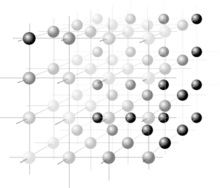
\includegraphics[width=0.4\textwidth]{220px-Voxelgitter.png}
 \caption{Illustration of a voxel grid containing color values}\cite[]{SHCHUROVA201576}
 \label{fig:voxel_repre} 
\end{figure}

This component of the PCL  framework aims to downsample (\textit{Reduce the Number of Points}) of a point cloud dataset using a voxelized grid method.
The \textbf{VoxelGrid} component, creates a 3D Voxel grid, which in common tearms refers to a set of small boxes in 3D space, over the input point cloud dataset. 
Once the its successfully converted into a voxel grid, then in each voxel(\textit{3D box}), all the existing points will be approximated (\textit{Downsampled}) with their centroid as suggested by \Citet*{Rusu_ICRA2011_PCL}.
This approach represents the underlaying surface of the point cloud dataset with high accuracy.
The main component is to set a defined and Voxel leaf Size, which allows to set the Voxel Size and the Number of Voxel in the Voxel Grid. Therefore, directly influencing the downsampling process and the resulting processed point cloud.

\subsection{Plane Model Segmentation}
%https://pcl.readthedocs.io/projects/tutorials/en/latest/planar_segmentation.html#planar-segmentation
This component of the PCL librabry aims to perform a plane segmentation of a given set of points, which finds all the points within a point cloud data set that support a plane model.
One of the components that this components uses is \textit{pcl::ExtractIndices}, which aims to extract thhe indices from a point cloud.
It is a filter that extracts a subset of points from a point cloud dataset, which are related to the indices output of a segmentation algorithm.

Similarly, it uses \textit{pcl::SACSegmentation}, which represents the Nodelet segmentation class for Sample Consensus methods and model, in a way that create a Nodelet wrapper which can be used
for generic-purpose SAC-based Segmentation \Citep*{Rusu_ICRA2011_PCL}.
The \textit{pcl::SACSegmentation}, creates an object and sets the model \& method type. Furthermore, it specifies the "distance threshold", that is used to determine the distance for point in the model, in order to be considered an inlier.
The used method in this project uses the \textbf{RANSAC} method. The main advantage of RANSAC is it's simplicity and robustness. 

The estimated plane parameters are estimated with equation \ref{equ:camera_intrisics}, where \textbf{a,b,c,d} are the model coefficient values.
\begin{equation}
  ax + by + cz + d = 0
\end{equation}
\label{equ:plane_param}

Figure \ref{fig:plane_seg}, illustrates the process below. The red points are the outliers, whereas the green points are the inliers of the found plane model.

\begin{figure}[H]%this figure will be at the right
  \centering
  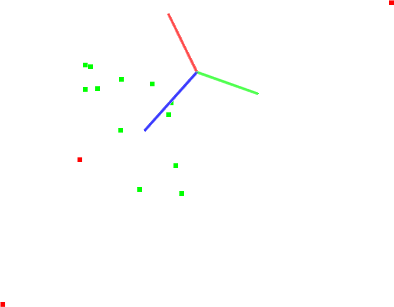
\includegraphics[width=0.4\textwidth]{planar_segmentation_2.png}
 \caption{Illustration of Plane model segmentation}\cite[]{SHCHUROVA201576}
 \label{fig:plane_seg} 
\end{figure}


\subsubsection*{RANSAC}
Random sample consensus (RANSAC), is an iterative method that is used to estimate parameters of a mathematical model from a set of observed data that contains outliers \Citep*{Strutz}.
Hence, it can be interpreted as an outlier detection method. It is an non-deterministic algorithm that generates an adequeate result with a specific probability,the probability increases as more iteration are performed.

\begin{figure}[H]%
  \centering
  \subfloat[\centering A data set with many outliers for which a line has to be fitted]{{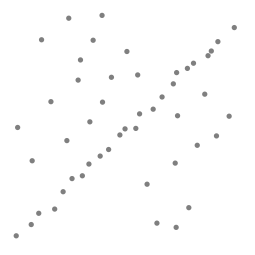
\includegraphics[width=5cm]{255px-Line_with_outliers.png} }}%
  \qquad
  \subfloat[\centering Fitted line with RANSAC; outliers have no influence on the result]{{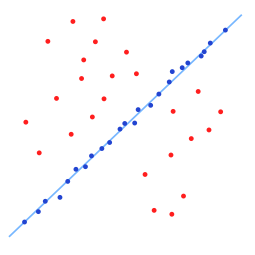
\includegraphics[width=5cm]{255px-Fitted_line.png} }}%
  \caption{Dataset Before \& After RANSAC algorithm \Citep*{Strutz}}%
  \label{fig:example}%
\end{figure}


\subsection {KdTree}
%https://pcl.readthedocs.io/projects/tutorials/en/latest/kdtree_search.html#kdtree-search
In this project Kdtrees are used to find the K nearest neighbour of certain points or locations and how to find these within an specified radius.

A K-D tree (\textit{k-dimensional tree}), is a data structure that is commonly used  to organize a certain number of points in a space with k dimensions as suggested by \Citet*{Rusu_ICRA2011_PCL}.
It is a binary search tree with other constrains imposed on it and are useful for searches for range and closest neighbours.
As this project uses pointclouds, the Kdtrees would have three dimensions. Each level of a Kdtree splits all children along a specific dimension, utilising a hyperplane which is perpendicular to the corresponding axis. 
At the root of the KdTree, all children will be divided based on the first dimension, and each level down in the Kdtree divides on the next dimension, finally it returns to the first dimension once 
all other have been exhausted \Citep*{Rusu_ICRA2011_PCL}.

KdTrees are used extensively in many components of the project framework pipeline.
\begin{figure}[H]%this figure will be at the right
  \centering
  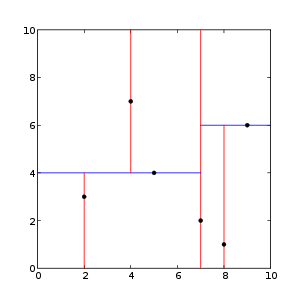
\includegraphics[width=0.4\textwidth]{2d_kdtree.png}
 \caption{Example of a 2-dimensional k-d tree}\cite[]{Rusu_ICRA2011_PCL}
 \label{fig:kdtree} 
\end{figure}

\subsection{Euclidean Cluster Extraction}
%https://pcl.readthedocs.io/projects/tutorials/en/latest/cluster_extraction.html?highlight=CLuster

The clustering method allows to divide a non-organized pointcloud dataset \textbf{$P$} into smaller components, in order to reduce the overall processing time for \textbf{$P$}.
Point Cloud Data Clustering can be approached in an Euclidean manner and be implemented using 3D grid subdivisions of the space with fixed width boxes or a octree data structure.
In this project, Kdtrees are used to find the nearest neighbours and implements a clustering technique which is similar to a flood fill algorithm \Citep*{Rusu_ICRA2011_PCL}.

The following Steps illustrates the clustering algorithm in this project with a Kdtree:

\begin{enumerate}
  \item create a Kd-tree representation for the input point cloud dataset $P$;
  \item set up an empty list of \textit{clusters} $C$, and a queue of the points that need to be checked $Q$;
  \item then for every point $p_i$ $\in$ $P$, perform the following steps:
  \begin{itemize}
    \item add $p_i$ to the current queue $Q$;
    \item for every point $p_i$ $\in$ $Q$ perform:
    \begin{itemize}
      \item Search for the set $P_{i}^{k}$ of point neighbors of $p_i$ in a sphere with radius $r$ $<$ $d_{th}$
      \item for every neighbor $p_{i}^{k}$ $\in$ $P_{i}^{k}$, check if the point has already been processed, and if not add it to $Q$
    \end{itemize}
    \item when the list of all points in $Q$ has been processed, add $Q$ to the list of clusters $C$, and reset $Q$ to an empty list

  \end{itemize}
  \item the algorithm terminates when all points $p_{i}^{k}$ $\in$ $P$ have been processed and are now part of the list of point clusters $C$
\end{enumerate}

Figure \ref{fig:cluster_example}, illustrates a cluustering output of a dataset, where different components were divided into multiple clusters
\begin{figure}[H]%this figure will be at the right
  \centering
  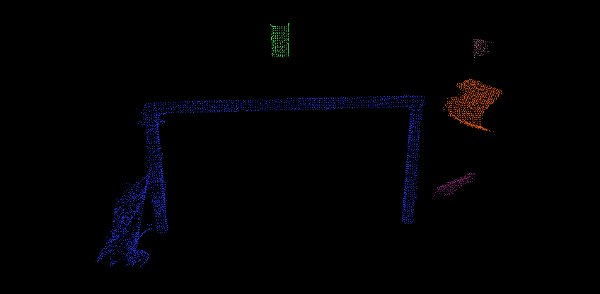
\includegraphics[width=1\textwidth]{cluster_extraction.jpg}
 \caption{Example of point clouud cluster}\cite[]{Rusu_ICRA2011_PCL}
 \label{fig:cluster_example} 
\end{figure}


\subsection{Principal Component Analysis}
%https://pointclouds.org/documentation/classpcl_1_1_p_c_a.html#details
The Principal Component Analysis (PCA) is the process of computing the principal components and use them to change the basis on data, using only the first few principal components
and discarding the rest. The principal components is a squence of $p$ unit vectors of a collection of points in a real coordinate space \Citep*{pca}.

The principal components are extracted using a singular value decomposition method, which is applied on the covarient matrix of the centered input point cloud dataset.
Once the PCA analysis is performed using the PCL library, it is possible to calculate the following components:
\begin{itemize}
  \item Mean of input data
  \item Eigen Vectors: Ordered set of vectors that represents the final principal components and the eigen cartesian space.
  \item Eigen Values: These are the correspondent loading of the Eigen Vectors ina decensing order.
\end{itemize}

The Principal Component Analysis is used to determine the scale of the Two point clouds that are used in this project and properly adjust the final mesh.

\subsection{Moving Least Squares }
%https://pcl.readthedocs.io/projects/tutorials/en/latest/resampling.html?highlight=smoothing
%https://pointclouds.org/documentation/classpcl_1_1_moving_least_squares.html
%https://pointclouds.org/documentation/classpcl_1_1_moving_least_squares.html#details
%http://alexandruichim.com/projects/tocs_final_ichim.pdf

Moving Least Squares (MLS) is a method of reconstructing continous functions from a set of unorganized point samples through the computation of weighted least squares, 
biased towards the region around the point at which the reconstructed value is requested \Citep*{mls}.

MLS can be modelled considering function $f$: $\mathbb{R}^n \rightarrow \mathbb{R}$ and a set of sample points $S = \{ ( x_i ; f_i ) | f(x_i) = f_i\} $.
Then, it MLS approximation of degree $m$ at the point $x$ is $\tilde{p} (x)$ where $\tilde{p}$ reduces the weighted least square error
$\sum_{i \in I} (p(x_i)-f_i)^2 \theta (\| x-x_i\| )$ over all polynomials $p$ of degree $m$ in $\mathbb{R}^n$ as mentioned by \Citet*{mls}.

The main objective of Moving Least Squares (MLS) is to smooth and resample noisy data in a surface reconstruction object.
Some pointclouds have certain data irregularities, which can be caused by small errors in the distances measurements, and are complex to remove using conventional
statistical analysis. It is important to account for complex surfaces and occlusions to create a complete model. Resampling algorithms such as MLS can be used to 
recreate the missing parts of the surface  by a high order polynomial interpolation between the surroundings data points.
Resampling, allows to correct the small errors and smooth the surface of a pointcloud dataset. 

\begin{figure}[H]%this figure will be at the right
  \centering
  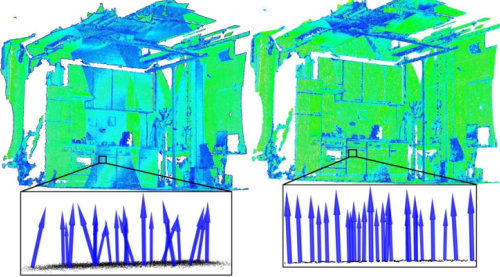
\includegraphics[width=0.7\textwidth]{resampling_1.jpg}
 \caption{Moving Least Square Smoothing}\cite[]{Rusu_ICRA2011_PCL}
 \label{fig:smoothing_mls} 
\end{figure}

On figure \ref{fig:smoothing_mls}, on the left side, it is illustrated the effect of estimating the normals of a pointcloud, however, due to alighment errors
the normals are noisy. On the right side of figure \ref{fig:smoothing_mls}, the effects of the MLS algorithm is demostrated as it smoothes the surface of the pointcloud.

In order to approximate, the surface illustrated by the local neighbours of points $p1,p2,....pk$ at a point $q$, it uses a bivariate polynomial function, which is defined on a robust modelled reference plane.
Figure \ref{fig:smoothing_curvature}, shows the curvatures at each point with the eigen value relation before and after the resampling method. 

\begin{figure}[H]%this figure will be at the right
  \centering
  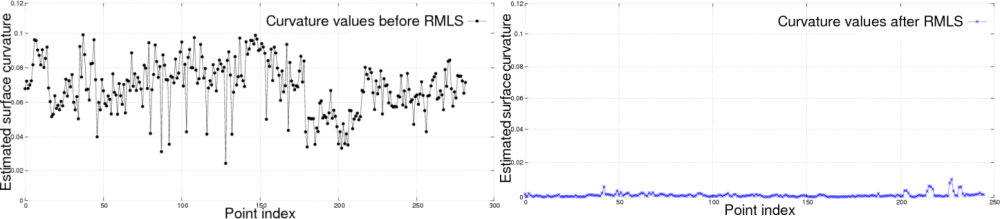
\includegraphics[width=1\textwidth]{resampling_2.jpg}
 \caption{Curvatures of MLS before \& after}\cite[]{Rusu_ICRA2011_PCL}
 \label{fig:smoothing_curvature} 
\end{figure}

Furthermore, the Moving Least Squares Component of the PCL library also allows for differnt upsample methods. 
These include 
\begin{description}
  \item[DISTINCT CLOUD] Project the points of the distinct cloud to the MLS surface\cite[]{Rusu_ICRA2011_PCL}.
  \item[SAMPLE LOCAL PLANE] The local plane of each input point will be sampled in a circular fashion using the $UpsamplingRadius$  and the $UpsamplingStep$ parameters\cite[]{Rusu_ICRA2011_PCL}. 
  \item[RANDOM UNIFORM DENSITY] The local plane of each input point will be sampled using an uniform random distribution such that the density of points is constant throughout the cloud - given by the $Desired Num Points in Radius Parameter$\cite[]{Rusu_ICRA2011_PCL}. 
  \item[VOXEL GRID DILATION] The input cloud will be inserted into a voxel grid with voxels of size $Voxel Size$.This voxel grid will be dilated $(Dilation Iteration Num)$ times and the resulting points will be projected to the MLS surface of the closest point in the input cloud; the result is a point cloud with filled holes and a constant point density \cite[]{Rusu_ICRA2011_PCL}.
\end{description}

For this project,  the \textbf {RANDOM UNIFORM DENSITY} method is used to upsample the MLS processed pointcloud. 
This method takes the parameters for a desired point cloud density within a fixed radius neighborhood as suggested by \Citet*{ichim_2012}. 
For each point, based on the density of the of the neighbors it will add more points on the local plane using a ramdom  number generator.
The random number generator will have a uniform distrubution and it will stop once the desired density is achived. Then it will replay the MLS algorithm in order to smooth the surface again.

Figure \ref{fig:sUpsample_def} illustrates on the left the implementation of MLS with \textbf{UNIFORM DENSITY} upsampling method on a pointcloud, whereas on the right  if the raw pointcloud.

\begin{figure}[H]%this figure will be at the right
  \centering
  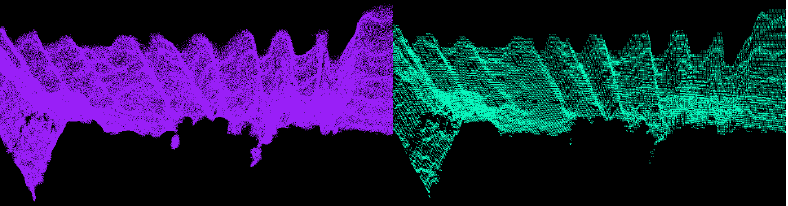
\includegraphics[width=1\textwidth]{upsample_def.png}
 \caption{Uniform Density Upsample Method After \& original}\cite[]{ichim_2012}
 \label{fig:sUpsample_def} 
\end{figure}


\subsection{Poisson Surface Reconstruction}
%https://pointclouds.org/documentation/classpcl_1_1_poisson.html#details
%https://pointclouds.org/documentation/classpcl_1_1_poisson.html
In this project the Poisson Reconstruction algorithm is implemented , to recontruct the processed point cloud.
The Poisson Reconstruction algorithm demostrates that the surface reconstruction from a set of oriented points can be associates as a spatial Poisson problem.
This formulation, utilizes all the points at once, with no need of using heuristic spatial partitioning or blending, hence, making it resilient to noise as mentioned by \Citet*{Poisson}.

The main objective of this algorithms to reconstruct a smooth surface, which is based on a large number of points $p_i$ from a pointcloud, where each point possesses an estimate of the local surface normal $n_i$
It aims to create an implicit function $f$, whose value is zero at the points $p_i$ and the gradient at points $p_i$ is equal to the normal vector $n_i$\Citet*{Poisson}.
The set of $(p_i,n_i)$ is modelled as a continouos vector field $V$ and the implicit function is found by integrating the vector field $V$.
In complex calculations, it is possible to perform a \textit{least-squares fit} to minimize the different between the gradient of $f$ and $V$\Citet*{Poisson}.



\begin{figure}[H]%this figure will be at the right
  \centering
  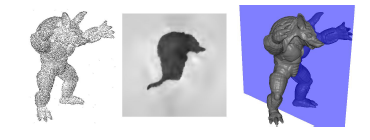
\includegraphics[width=1\textwidth]{poisson_example.png}
 \caption{Poisson Recontruction Example. On the left it it input pointcloud dataset, whereas on the right is output of the Poisson Surface Reconstruction Algorithm}\cite[]{Poisson}
 \label{fig:Poisson_def} 
\end{figure}



\section{Open3D}
Open3D is an open source library that supports fast development of software that handles 3D data.
The Open3D frontend exposes outputs a set of carefully choosen data structures and algorithms in both Python and C++ \Citep*{Zhou2018}. 
The backend of the framework is highly optimized and it configured for parallelization.
Open3D is compatible with Linux, macOS and Windows and it can be installed via source of via packages. 

The core features include: 
\begin{multicols}{2}
  \begin{itemize}
    \item Simple installation via conda and pip
    \item 3D data structures
    \item 3D data processing algorithms
    \item Scene reconstruction
    \item Surface alignment
    \item PBR rendering
    \item 3D visualization
    \item Python binding
  \end{itemize}
  \end{multicols}


In this project Open3D was used as an axiliary library used as contingency for Poisson Reconstruction. 
As in many circumstances the normals of a Pointcloud, might not be properly oriented \textit{orient normals consistent tangent plane} allows to propagate the normal orientation with a minimum
spanning tree as suggested by \Citet*{Zhou2018}. 
After the normals is aligned it will  excute the Poission Surface Recontruction algorithm \Citep*{Poisson} and solves a regularized optimization problem to obtain a smooth surface mesh. 


\begin{figure}[H]%this figure will be at the right
  \centering
  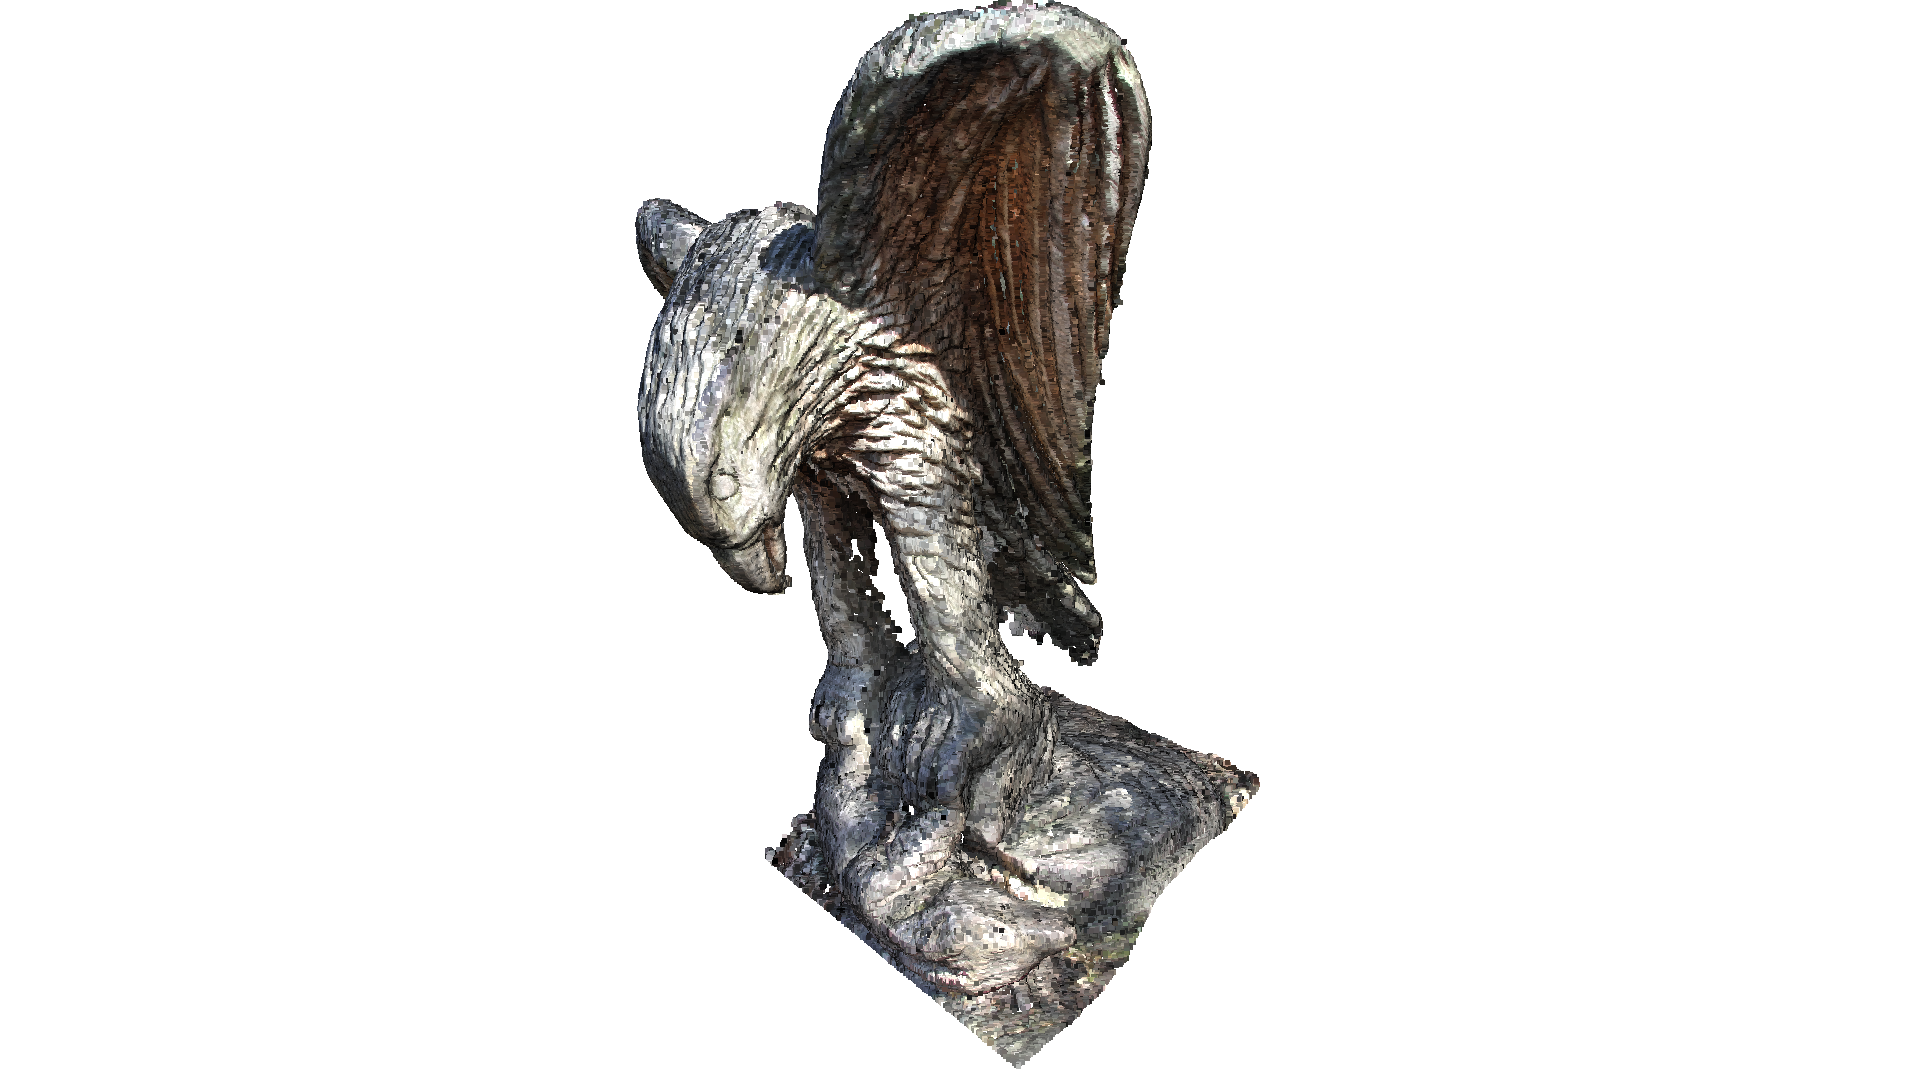
\includegraphics[width=1\textwidth]{open3dpoisson.png}
 \caption{Open3D Poisson Recontruction Example}\cite[]{Zhou2018}
 \label{fig:Possion_exampple} 
\end{figure}



\chapter{Methodology}
As mentioned before, this project is associated with the software reconstruction of a 3D scanner device.
The key components are divided into three processes that include:

\begin{itemize}
  \item Data collection
  \item Photogrammetry Process
  \item Point Cloud Processsing \& Reconstruction
\end{itemize}

All the components mentioned above will work in a Pipeline manner and as the key process for a 3D scanner includes the Data collection. 
Once the Data is collected, a protogrammetry process will run in order to reconstruct the object based on the input data. 
Finally, the resultant reconstructed object will be processed using a Custom framework pipeline based on the PCL (\textit{Point Cloud Library}) and procede a processed mesh.
Once the mesh has finished processing it can be used in different applications such as clothes fitting, etc.

\section{Data Collection}
The data Collection process is perform with a 3D scanning RIG (device).
The process will be perform with a series of twenty-eight cameras and a single Lidar. 
The cameras will be located and assembled in a series of eight tall poles and 4 short poles. Similarly, the Lidar will be mounted to a single Pole.

All  the cameras will be controlled using Raspberry Pis.
There will be a total of three Raspberry Pi's that set the excution process to acquire data from all the cameras that are attached to them, with a total number of twenty eight images
Similarly, an Nvidia Jetson Xavier is used to acquire data from the Lidar. The Nvidia Jetson Xavier will acquire a single image an a PointCloud of the scanned subject. 

\newpage
\subsubsection*{Cameras}

 
\begin{wrapfigure}[7]{r}{0.2\textwidth}
  \begin{center}
    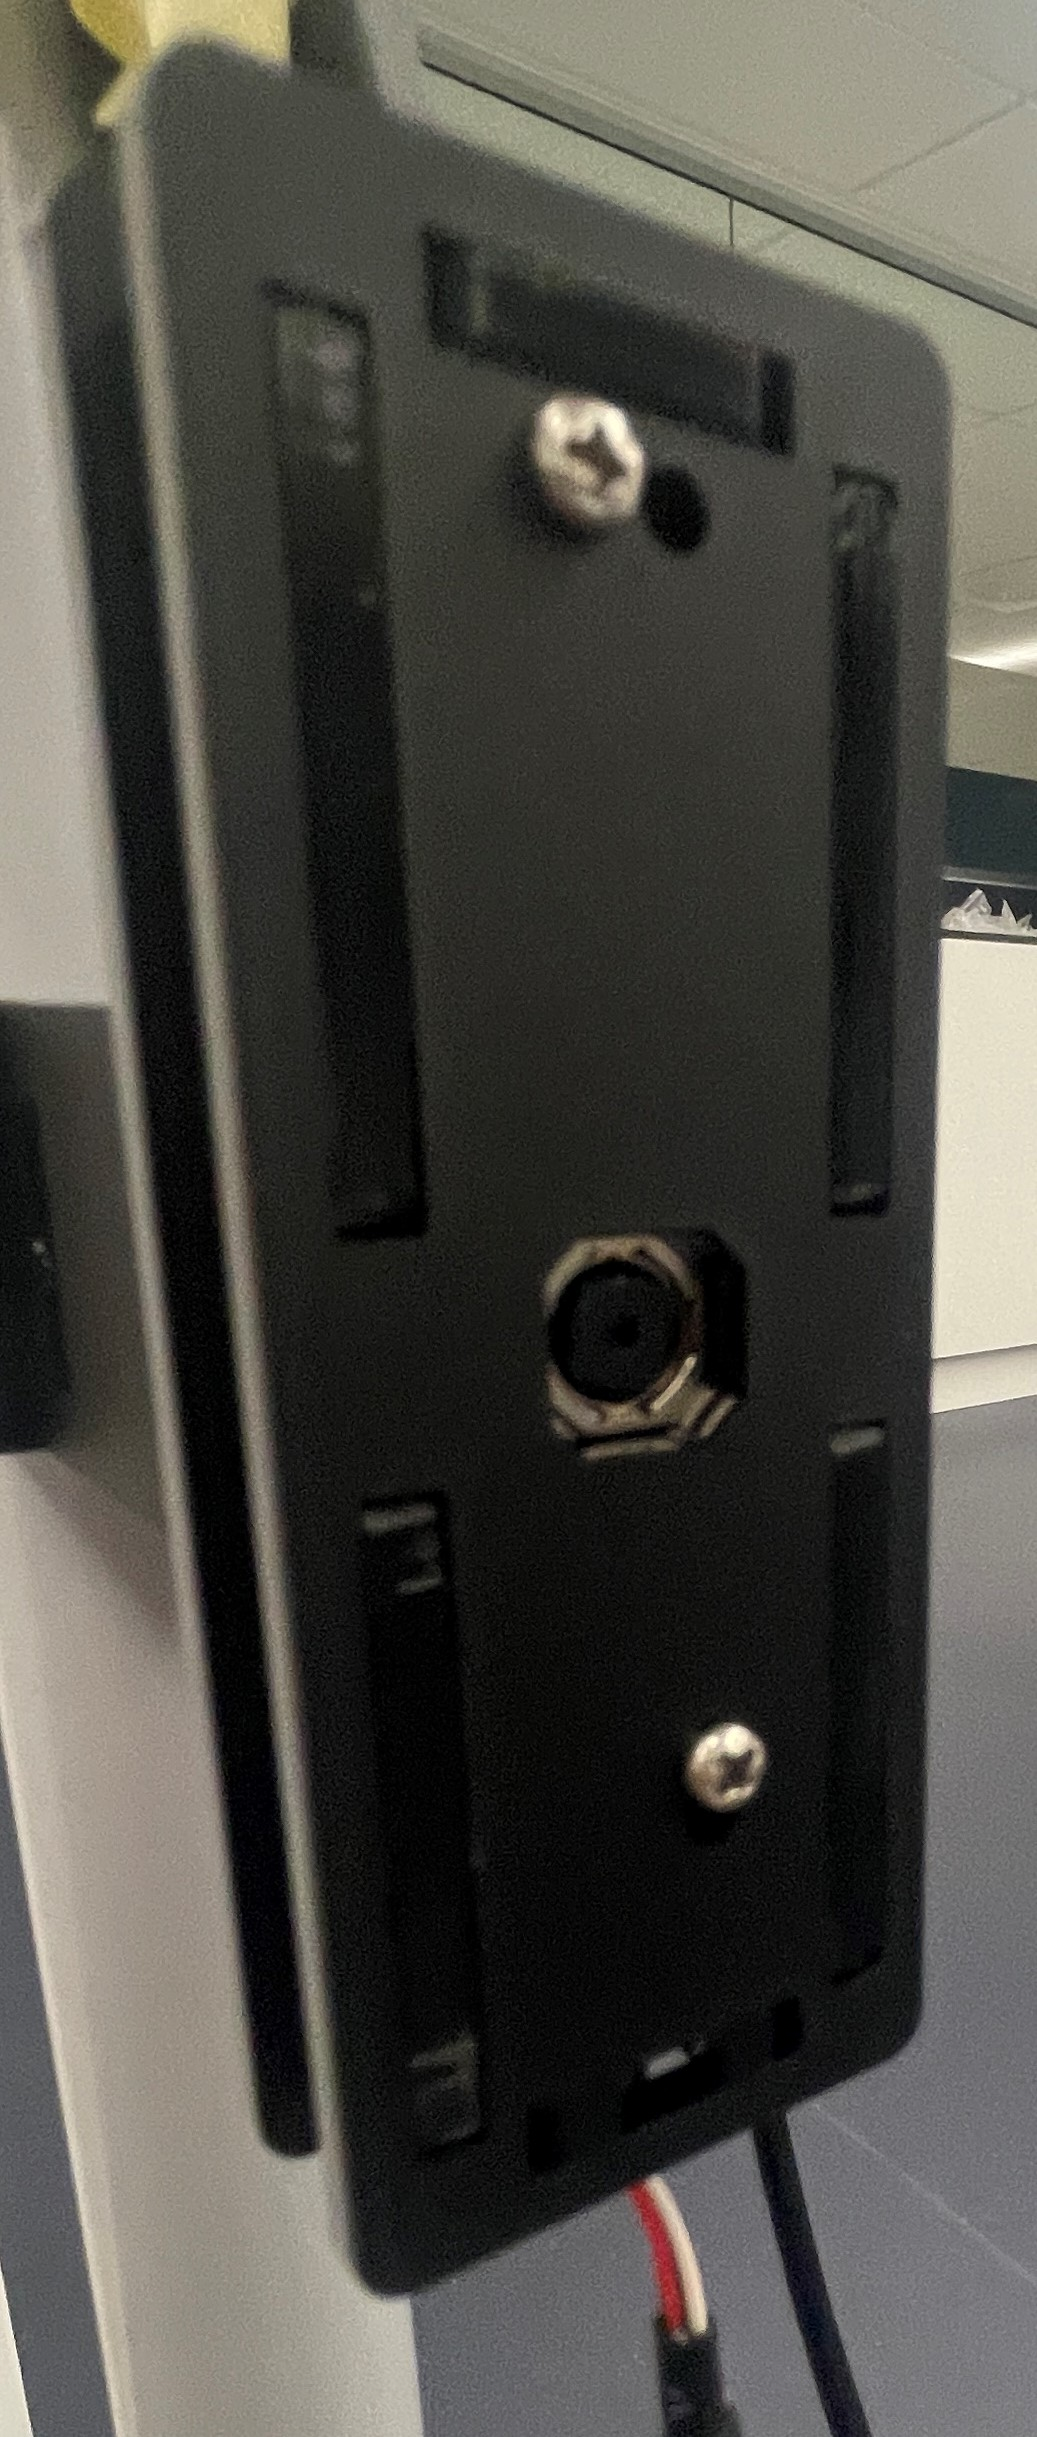
\includegraphics[width=0.2\textwidth]{IMG_5885_cropped.jpg}
  \end{center}
  \vspace{-10pt}
  \caption{Tall Pole Cameras Location With Housing.}
  \label{fig:Cameras}
\end{wrapfigure}

The cameras used for data acquisition have the following specifications. 
\begin{table}[H]
  %  \centering
  \begin{tabular}{|l|l|}
  \hline
  Model No.         & HBV-1825                         \\ \hline
  Model Size        & 62mm × 9mm × 5.68mm±0.2mm        \\ \hline
  Active Array Size & 2592 x 1944                      \\ \hline
  Pixel Size        & 1.4µm x1.4µm                     \\ \hline
  shutter           & rolling shutter / frame exposure \\ \hline
  Field of View     & 65°                              \\ \hline
  \end{tabular}
  \captionsetup{singlelinecheck = false, format= hang, justification=raggedright, font=footnotesize, labelsep=space}
  \caption{Cameras Specification}
  \label{tab:Cameras_specs}
\end{table}

As observed in figure \ref{fig:Cameras}, the cameras will have a Plastic Housing. This Housing device allows to safely place the cameras 
in the poles as well as protecting the electronics and connection from external factors.
The cameras will be connected to a series of USB hubs that will be directly connected to the Raspberry Pi's to control the data acquisition process.

\subsubsection*{Lidar}

\begin{wrapfigure}[10]{l}{0.2\textwidth}
  \begin{center}
    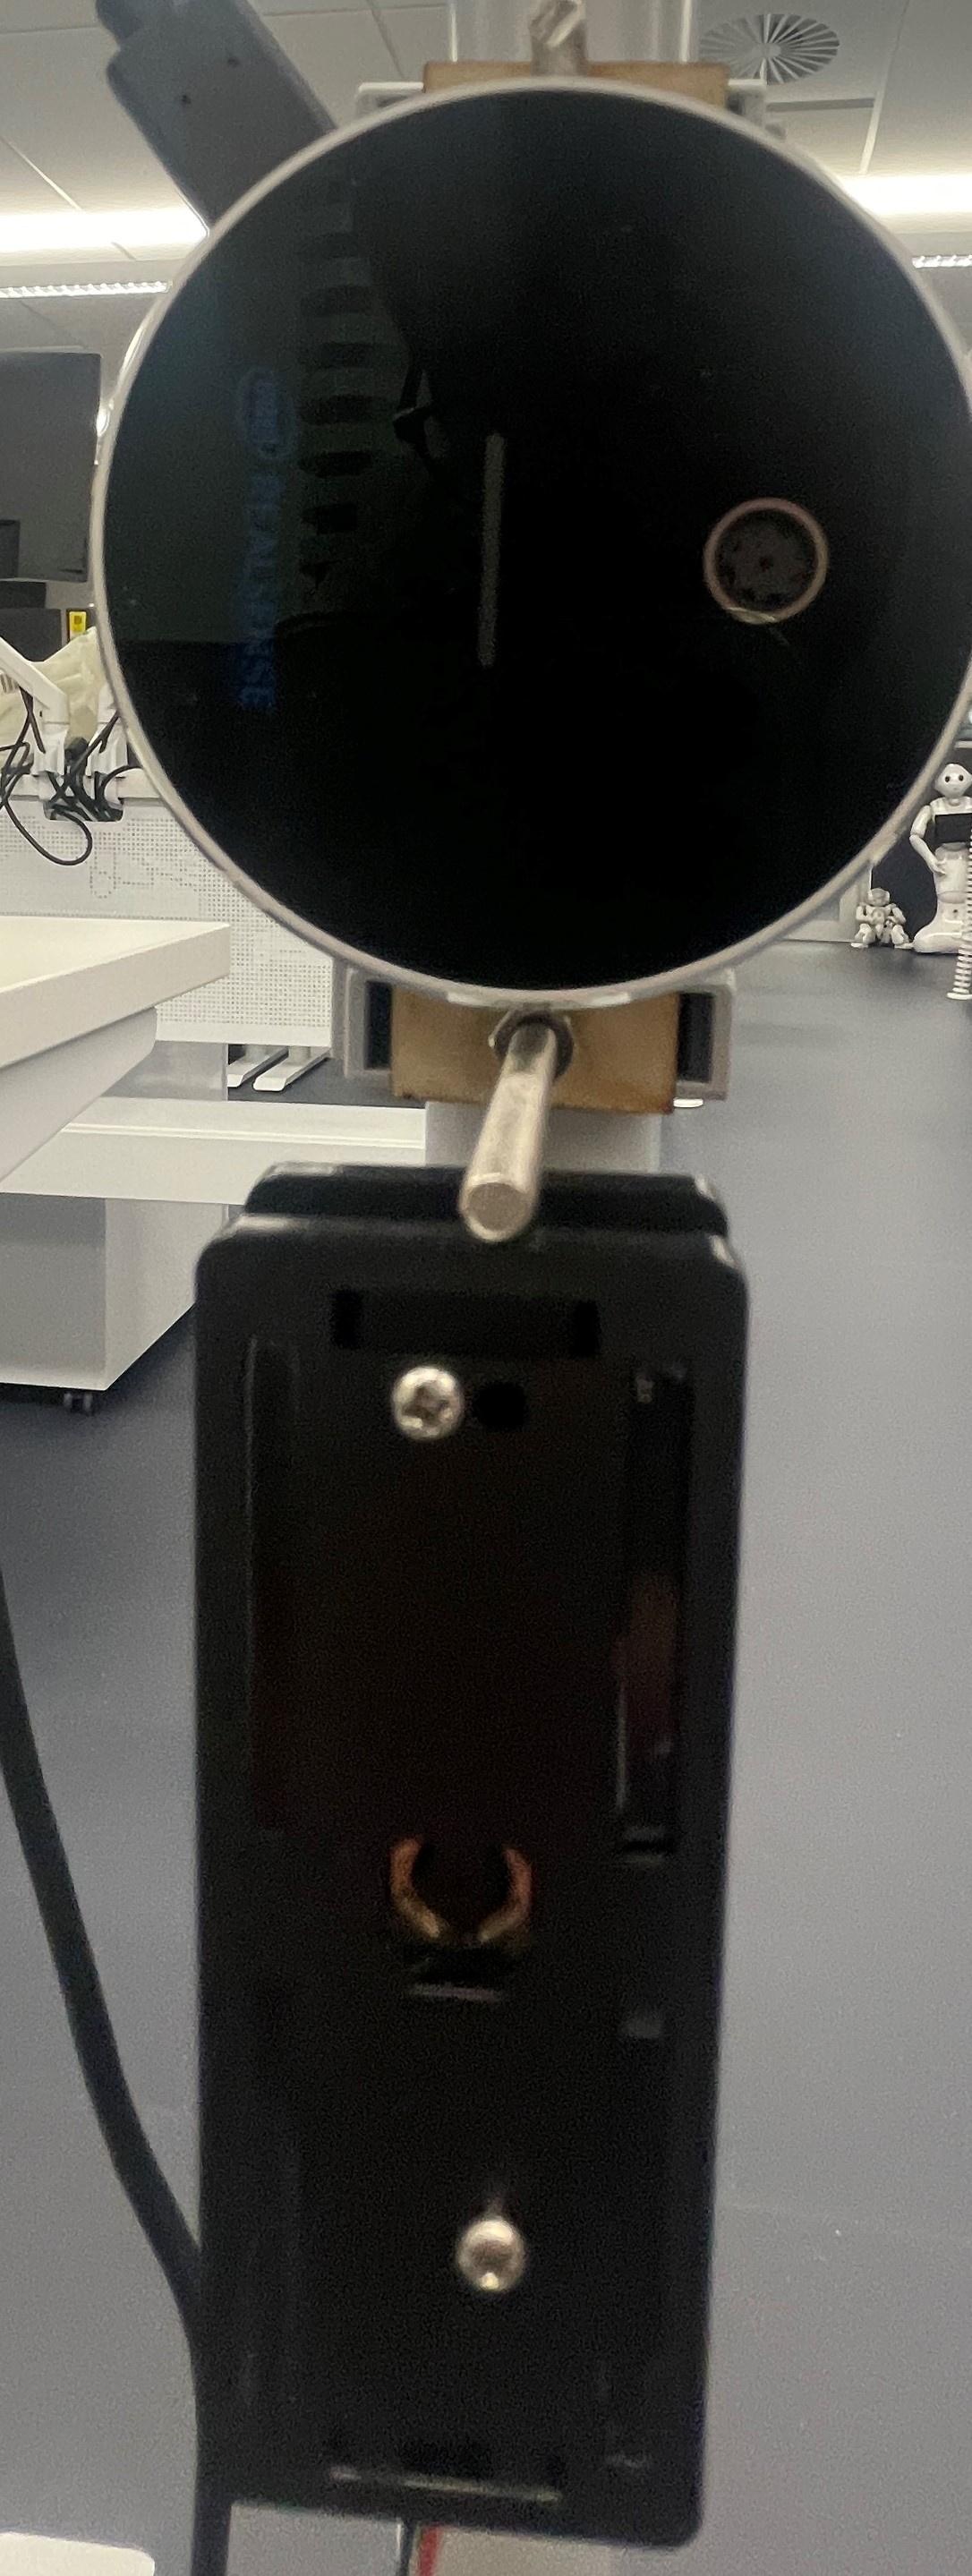
\includegraphics[width=0.2\textwidth]{IMG_5886_cropped.jpg}
  \end{center}                          
  \caption{Lidar Mounted in Pole}
  \label{fig:lidar_mounted}
\end{wrapfigure}
The Lidar used for the data acquisition process in an Intel RealSense L515.
The Intel RealSense will be located in tall pole and it will be attached in the middle section in order to maximise the field of view. It will be locked above the middle camera of a tall pole.
As the Lidar has both an RGB sensor and a Depth Camera, it will be used to capture an RGB image as well as a Pointcloud with the Depth and RGB Sensor.
The Lidar will be connected and controlled with a Nvidia Jetson Xavier. It will use the RealSense SDK to capture both RGB image and Point.

Table \ref{tab:lidar_specs} states the specification of the Intel RealSense L515. 

\begin{table}[H]
    \centering
    \begin{tabular}{|l|l|}
    \hline
    Model No.                  & Intel RealSense L515               \\ \hline
    Depth Technology           & Lidar                              \\ \hline
    Ideal Range                & 0.25 m to 9 m                      \\ \hline
    Depth Field of View (FOV): & 70° × 55° (±3°)                    \\ \hline
    Depth output resolution:   & Up to 1024 × 768                   \\ \hline
    Depth Accuracy:            & $\sim$5 mm to $\sim$14 mm thru 9 m \\ \hline
    RGB frame resolution       & 1920 × 1080                        \\ \hline
    RGB sensor technology      & Rolling Shutter                    \\ \hline
    RGB sensor FOV (H × V)     & 70° × 43° (±3°)                    \\ \hline
    RGB sensor resolution      & 2 MP                               \\ \hline
    \end{tabular}
    \caption{Intel RealSense L515 Specification}
    \label{tab:lidar_specs}
\end{table}

\subsection{Layout \& Configuration}
As mentioned before Lidar will be controlled to an Nvidia Jetson Xavier, which will make it agnostic of the Cameras acquisition process. 
It was previously mentioned that the Cameras will be controlled with a Series of multiple Raspberry Pi's and those will be managed via a SSH connection with Putty. 
Due to the limited number of USB connectors, a series of USB hubs will be used in order to control more cameras with Single Raspberry Pi's.
Figure \ref{fig:cameras_layout}, illustrates how the twenty-eight cameras will be connected with the Different Raspberry Pi's.

\begin{figure}[H]%this figure will be at the right
   \centering
  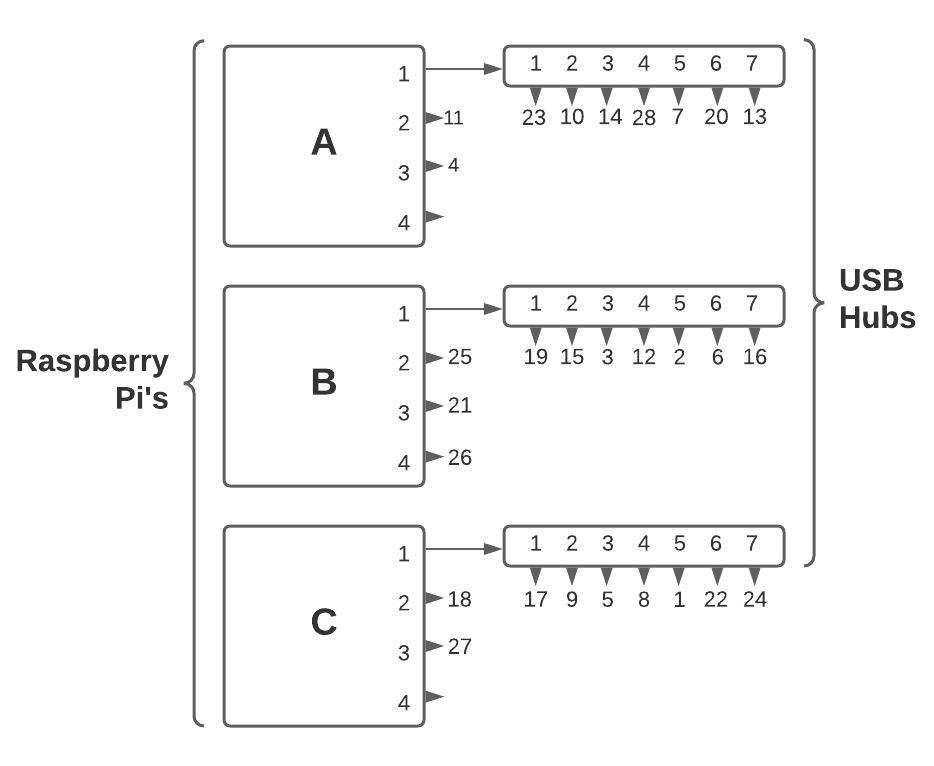
\includegraphics[width=0.6\textwidth]{cameras_layout.png}
 \caption{Cameras Lay-out connection}
 \label{fig:cameras_layout} 
\end{figure}


\begin{wrapfigure}[17]{r}{0.3\textwidth}
  \begin{center}
    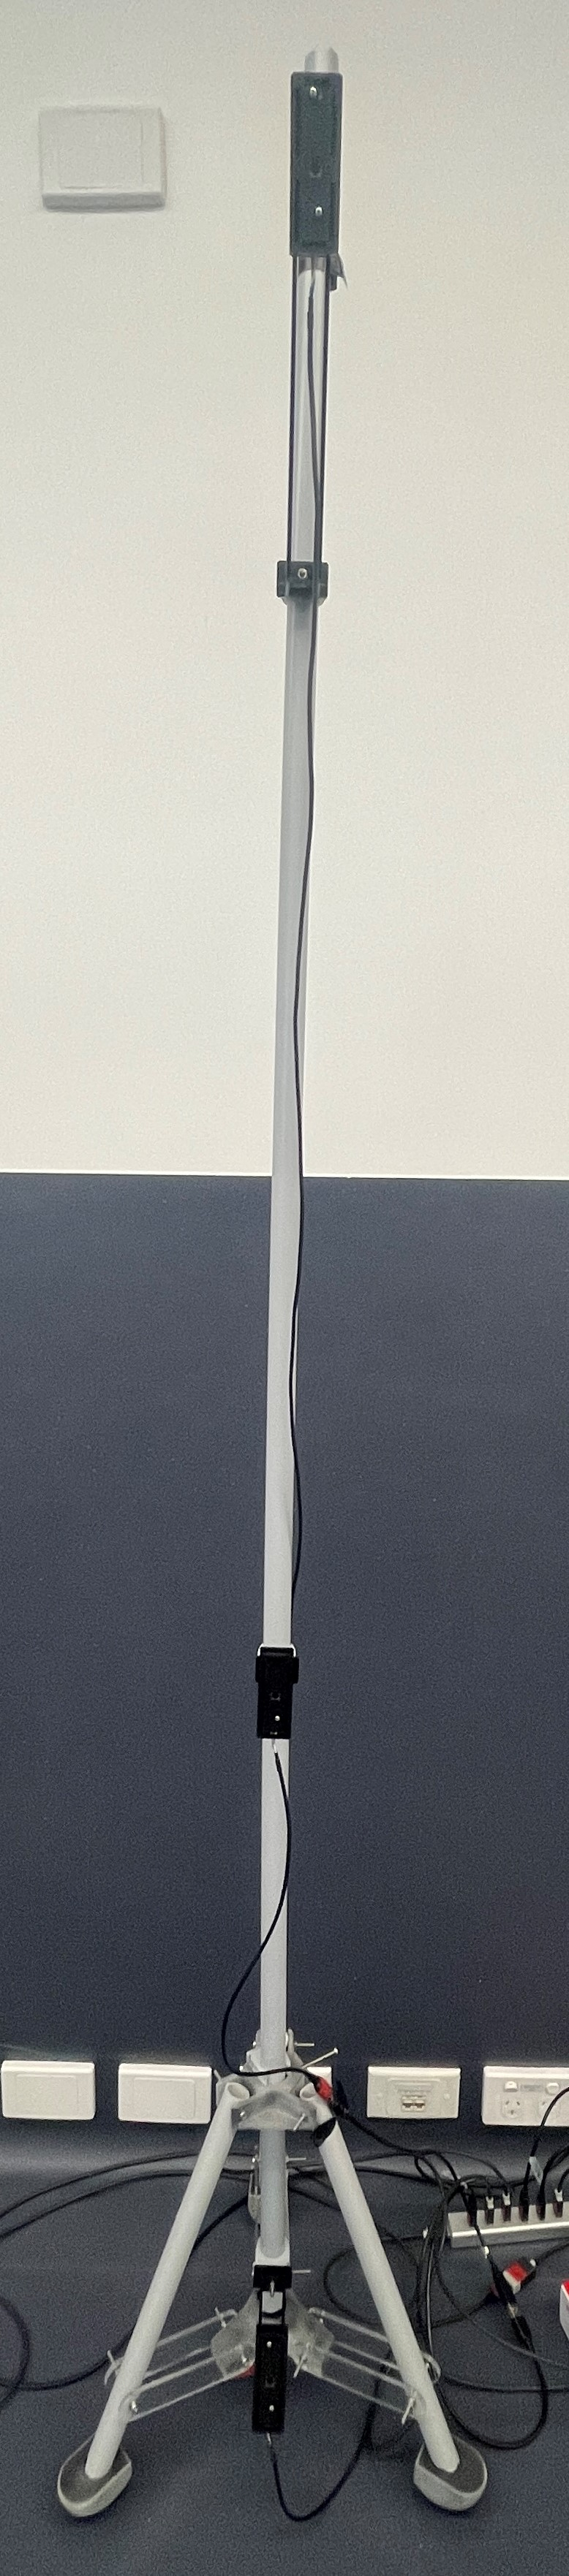
\includegraphics[width=0.25\textwidth]{IMG_5895_cropped.jpg}
  \end{center}
  \caption{Tall Pole Cameras Configuration.}
  \label{fig:poles_camera_tall}
\end{wrapfigure}
All the cameras will be mounted in the RIG in a series of Pole. There will be a total number of eight tall and four short poles.
The Tall Poles will be used to attached three cameras to the Frame. The First Camera will be located on top of the pole and oriented toward the subject in order to have the best overlap with the Field of View.
The Second Camera is located in the middle of the pole and parallel oriented to the scanned subject in order to have the best field of view. 
The third Camera is located at the bottom of the pole and it will oriented upwards toward the scanned subject in order to have the a wide coverage. 
This configuration can be observed on figure \ref{fig:poles_camera_tall}.

On the other side, there will be four short poles that each will hold a single camera. 
The aim of these poles is to gain close data as well as acquiring images from regions of interest around the body in order to increases
the accuracy of the final scan. 

\begin{figure}[H]
  % \raggedright
  \hspace*{0.8cm}  
  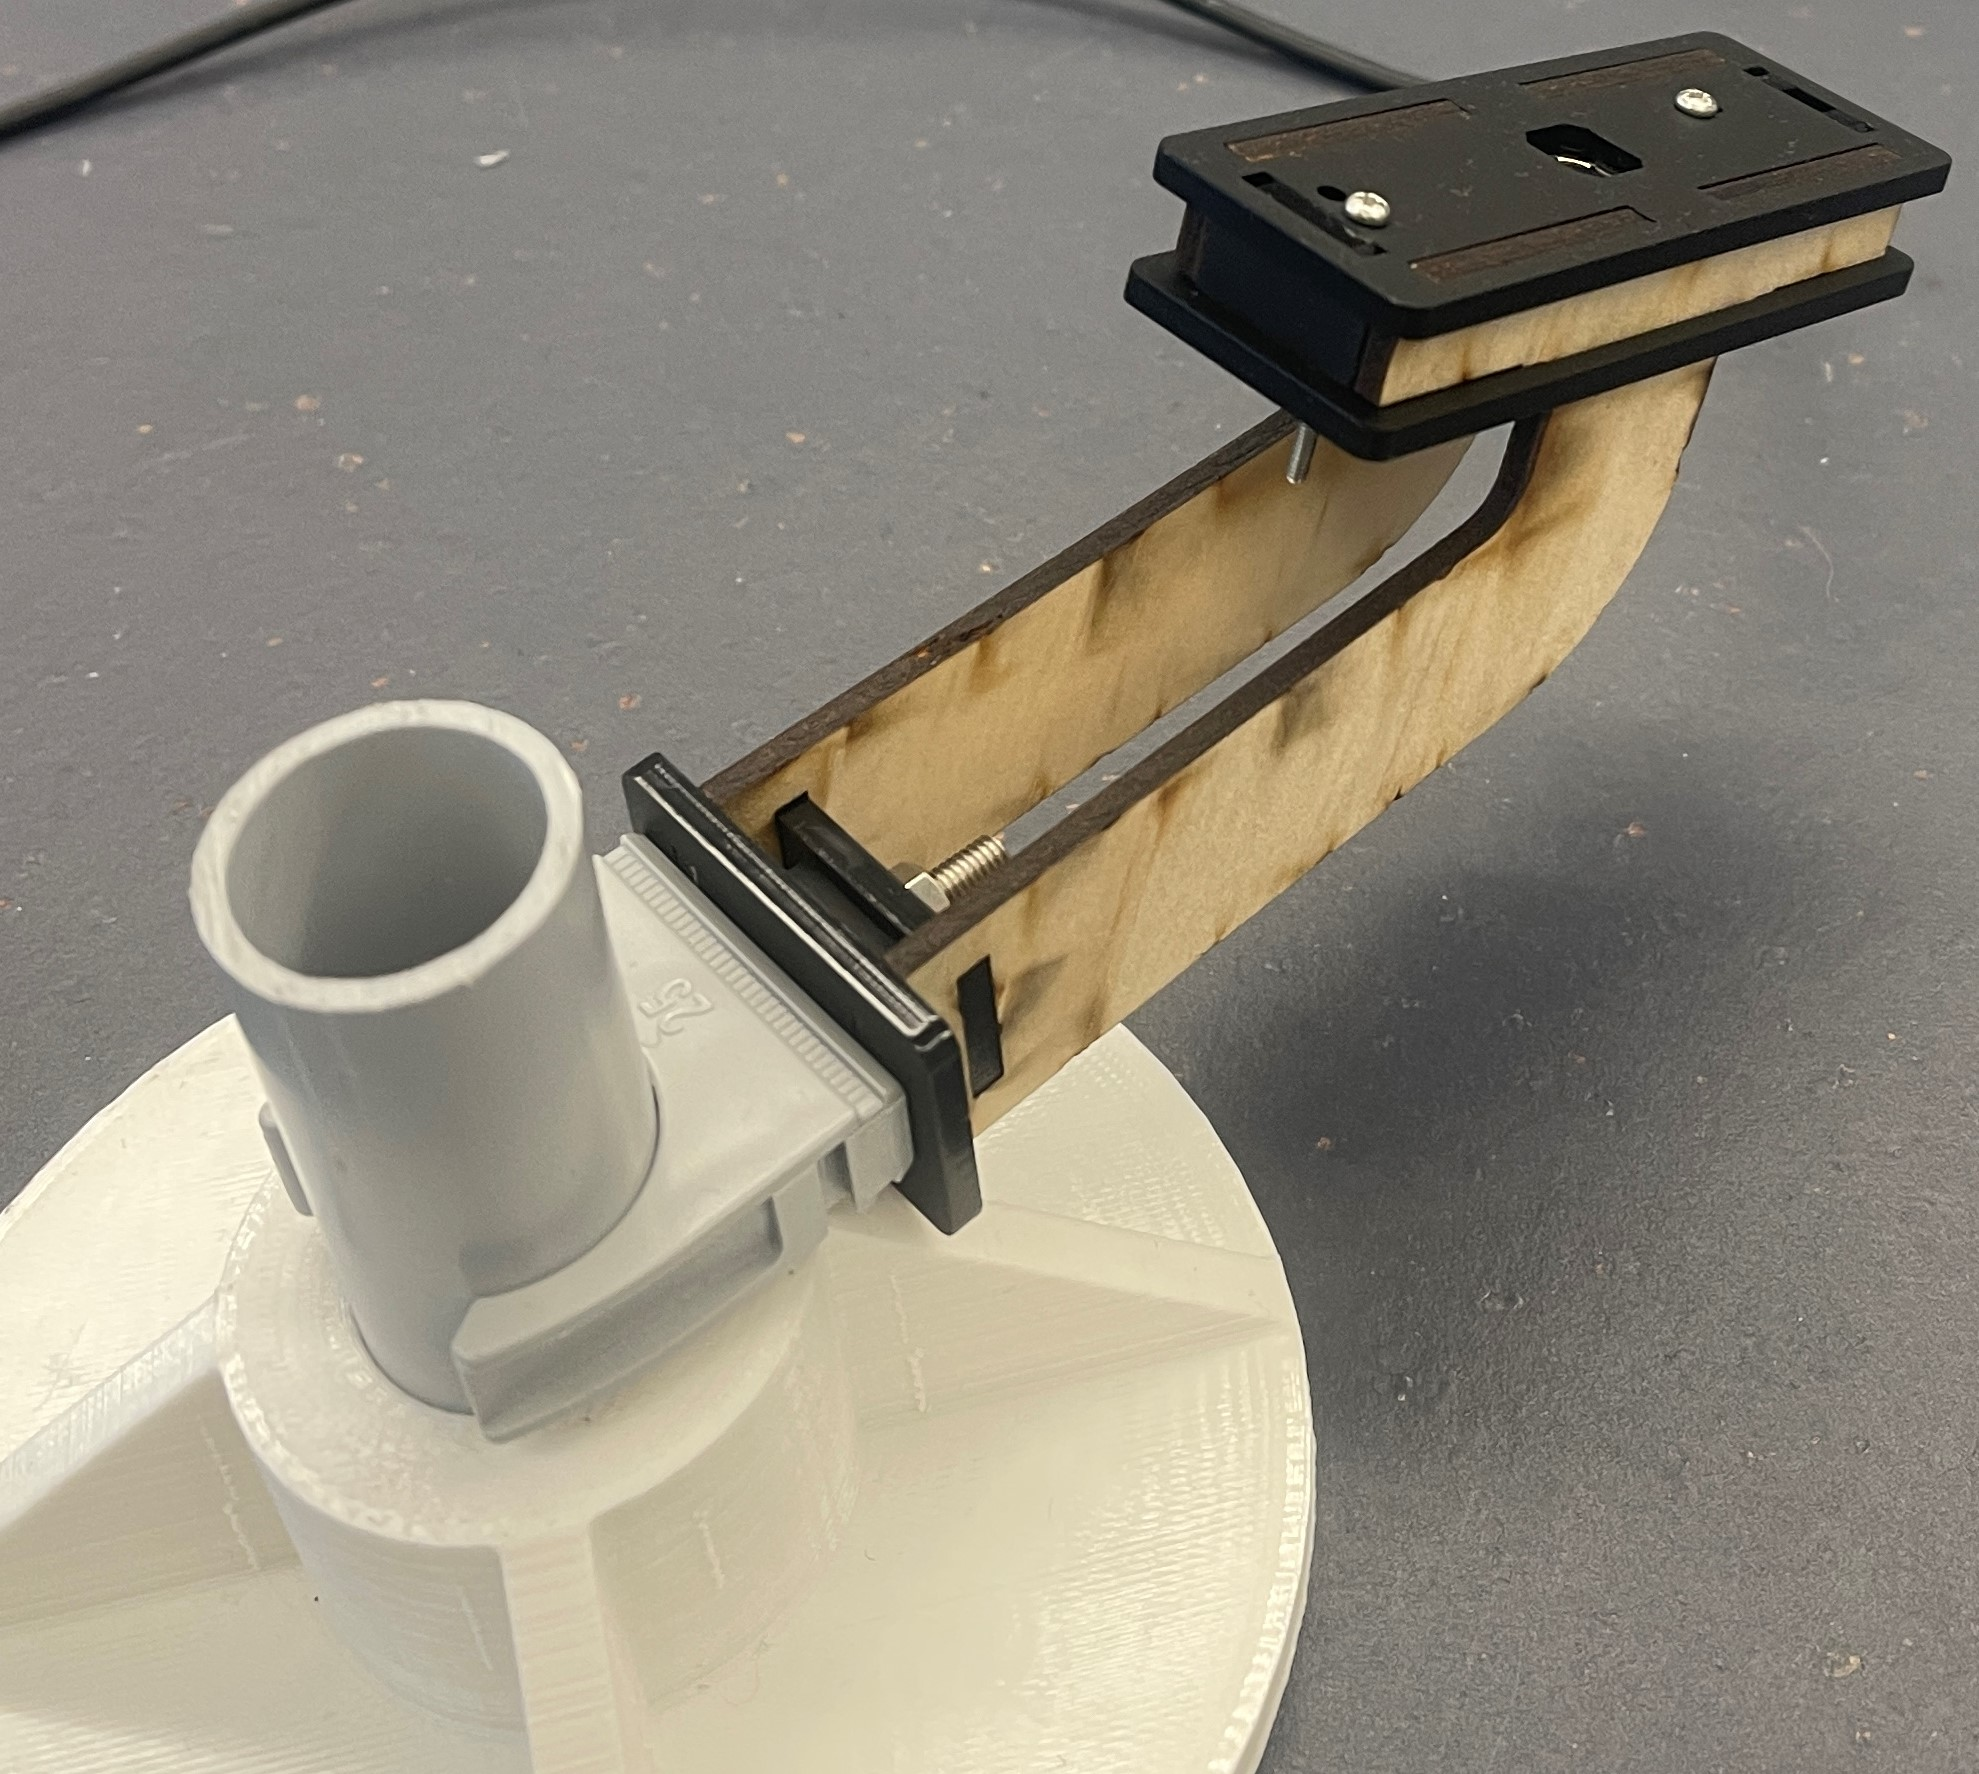
\includegraphics[width=0.5\textwidth]{IMG_5896_cropped.jpg}
  \captionsetup{singlelinecheck = false, format= hang, justification=raggedright,  labelsep=space}
 \caption{Open3D Poisson Recontruction Example}
 \label{fig:short_pole} 
\end{figure}

All the tall poles will be placed in a circular shape in order to capture as much data as possible. 
The subject (person) that will use the RIG will be located in the origin of the circle and all the tall poles will be places at a 1.5 m away from the person in order to have the best overlap between all cameras.
The four short poles will be located closeup from the person that will be scanned. The four poles will be placed at 60 cm away from the person (circle origin) in order to capture close up data for complex regions and improve the overall reconstruction.
\enlargethispage{\baselineskip}

\newpage


\begin{figure}[H]
  \centering
  \subfloat[RIG From View]{{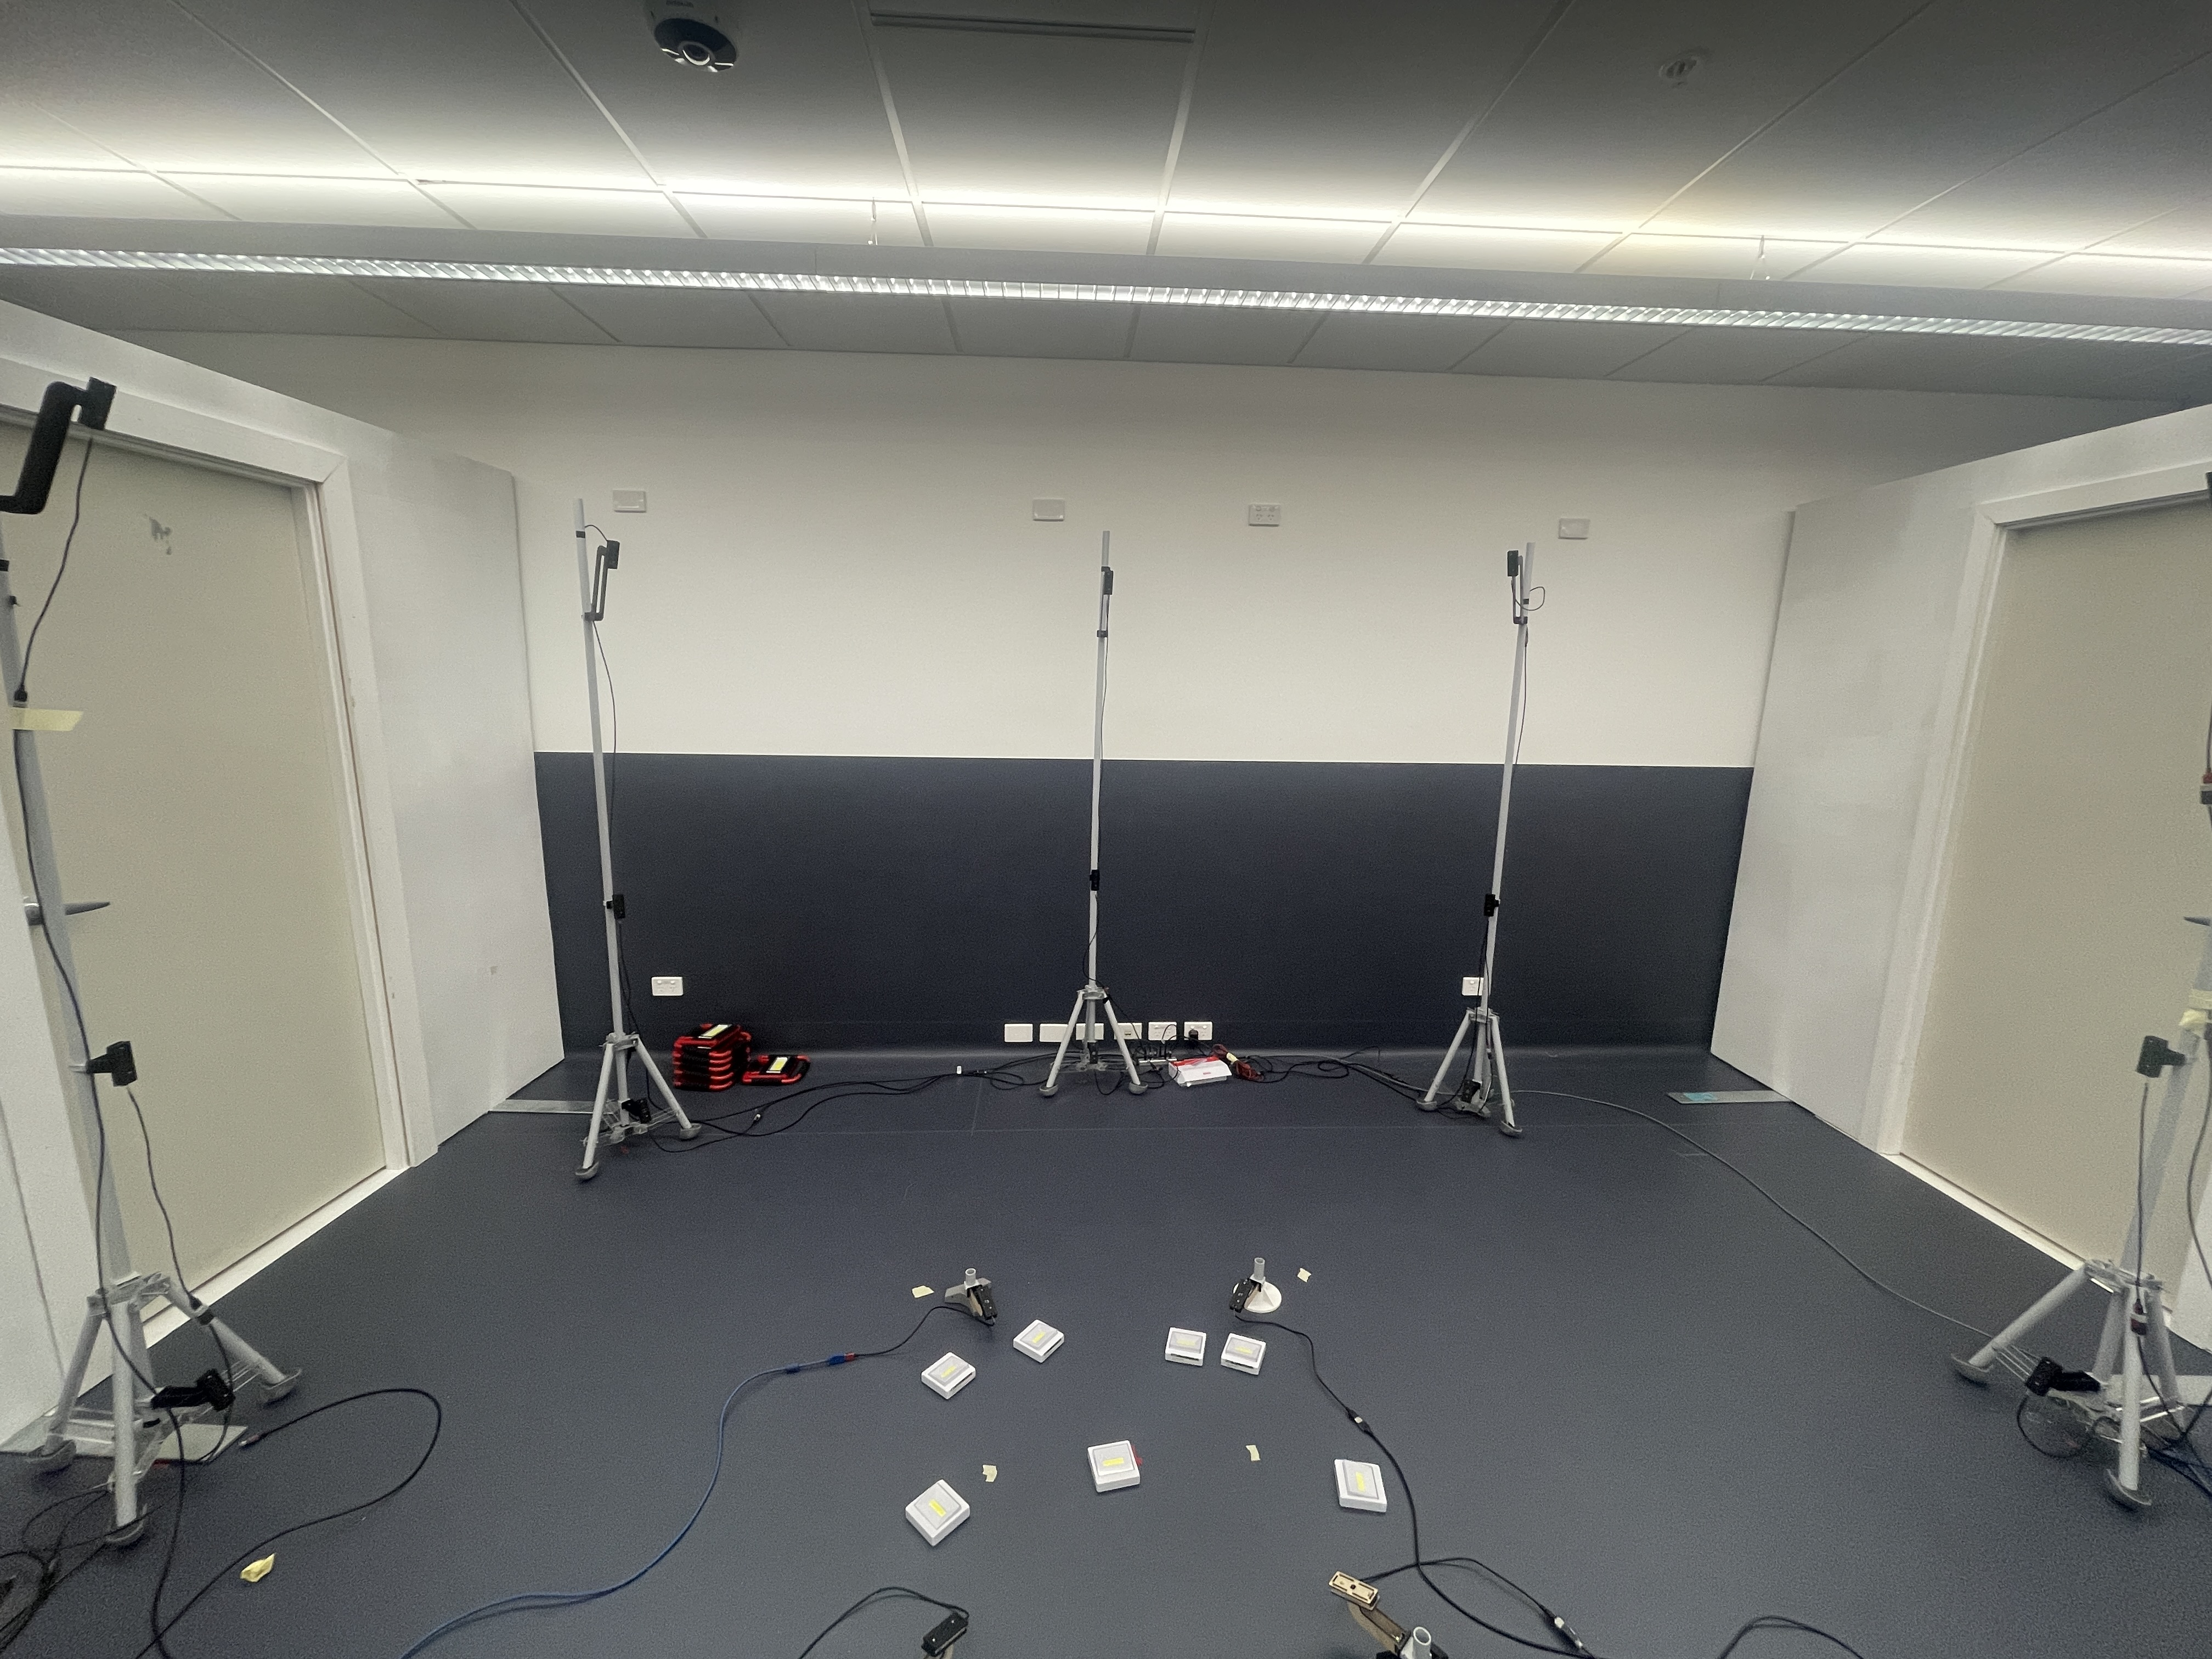
\includegraphics[width=0.85\textwidth]{IMG_5883.JPG} }}
  \qquad
  \subfloat[RIG lateral View]{{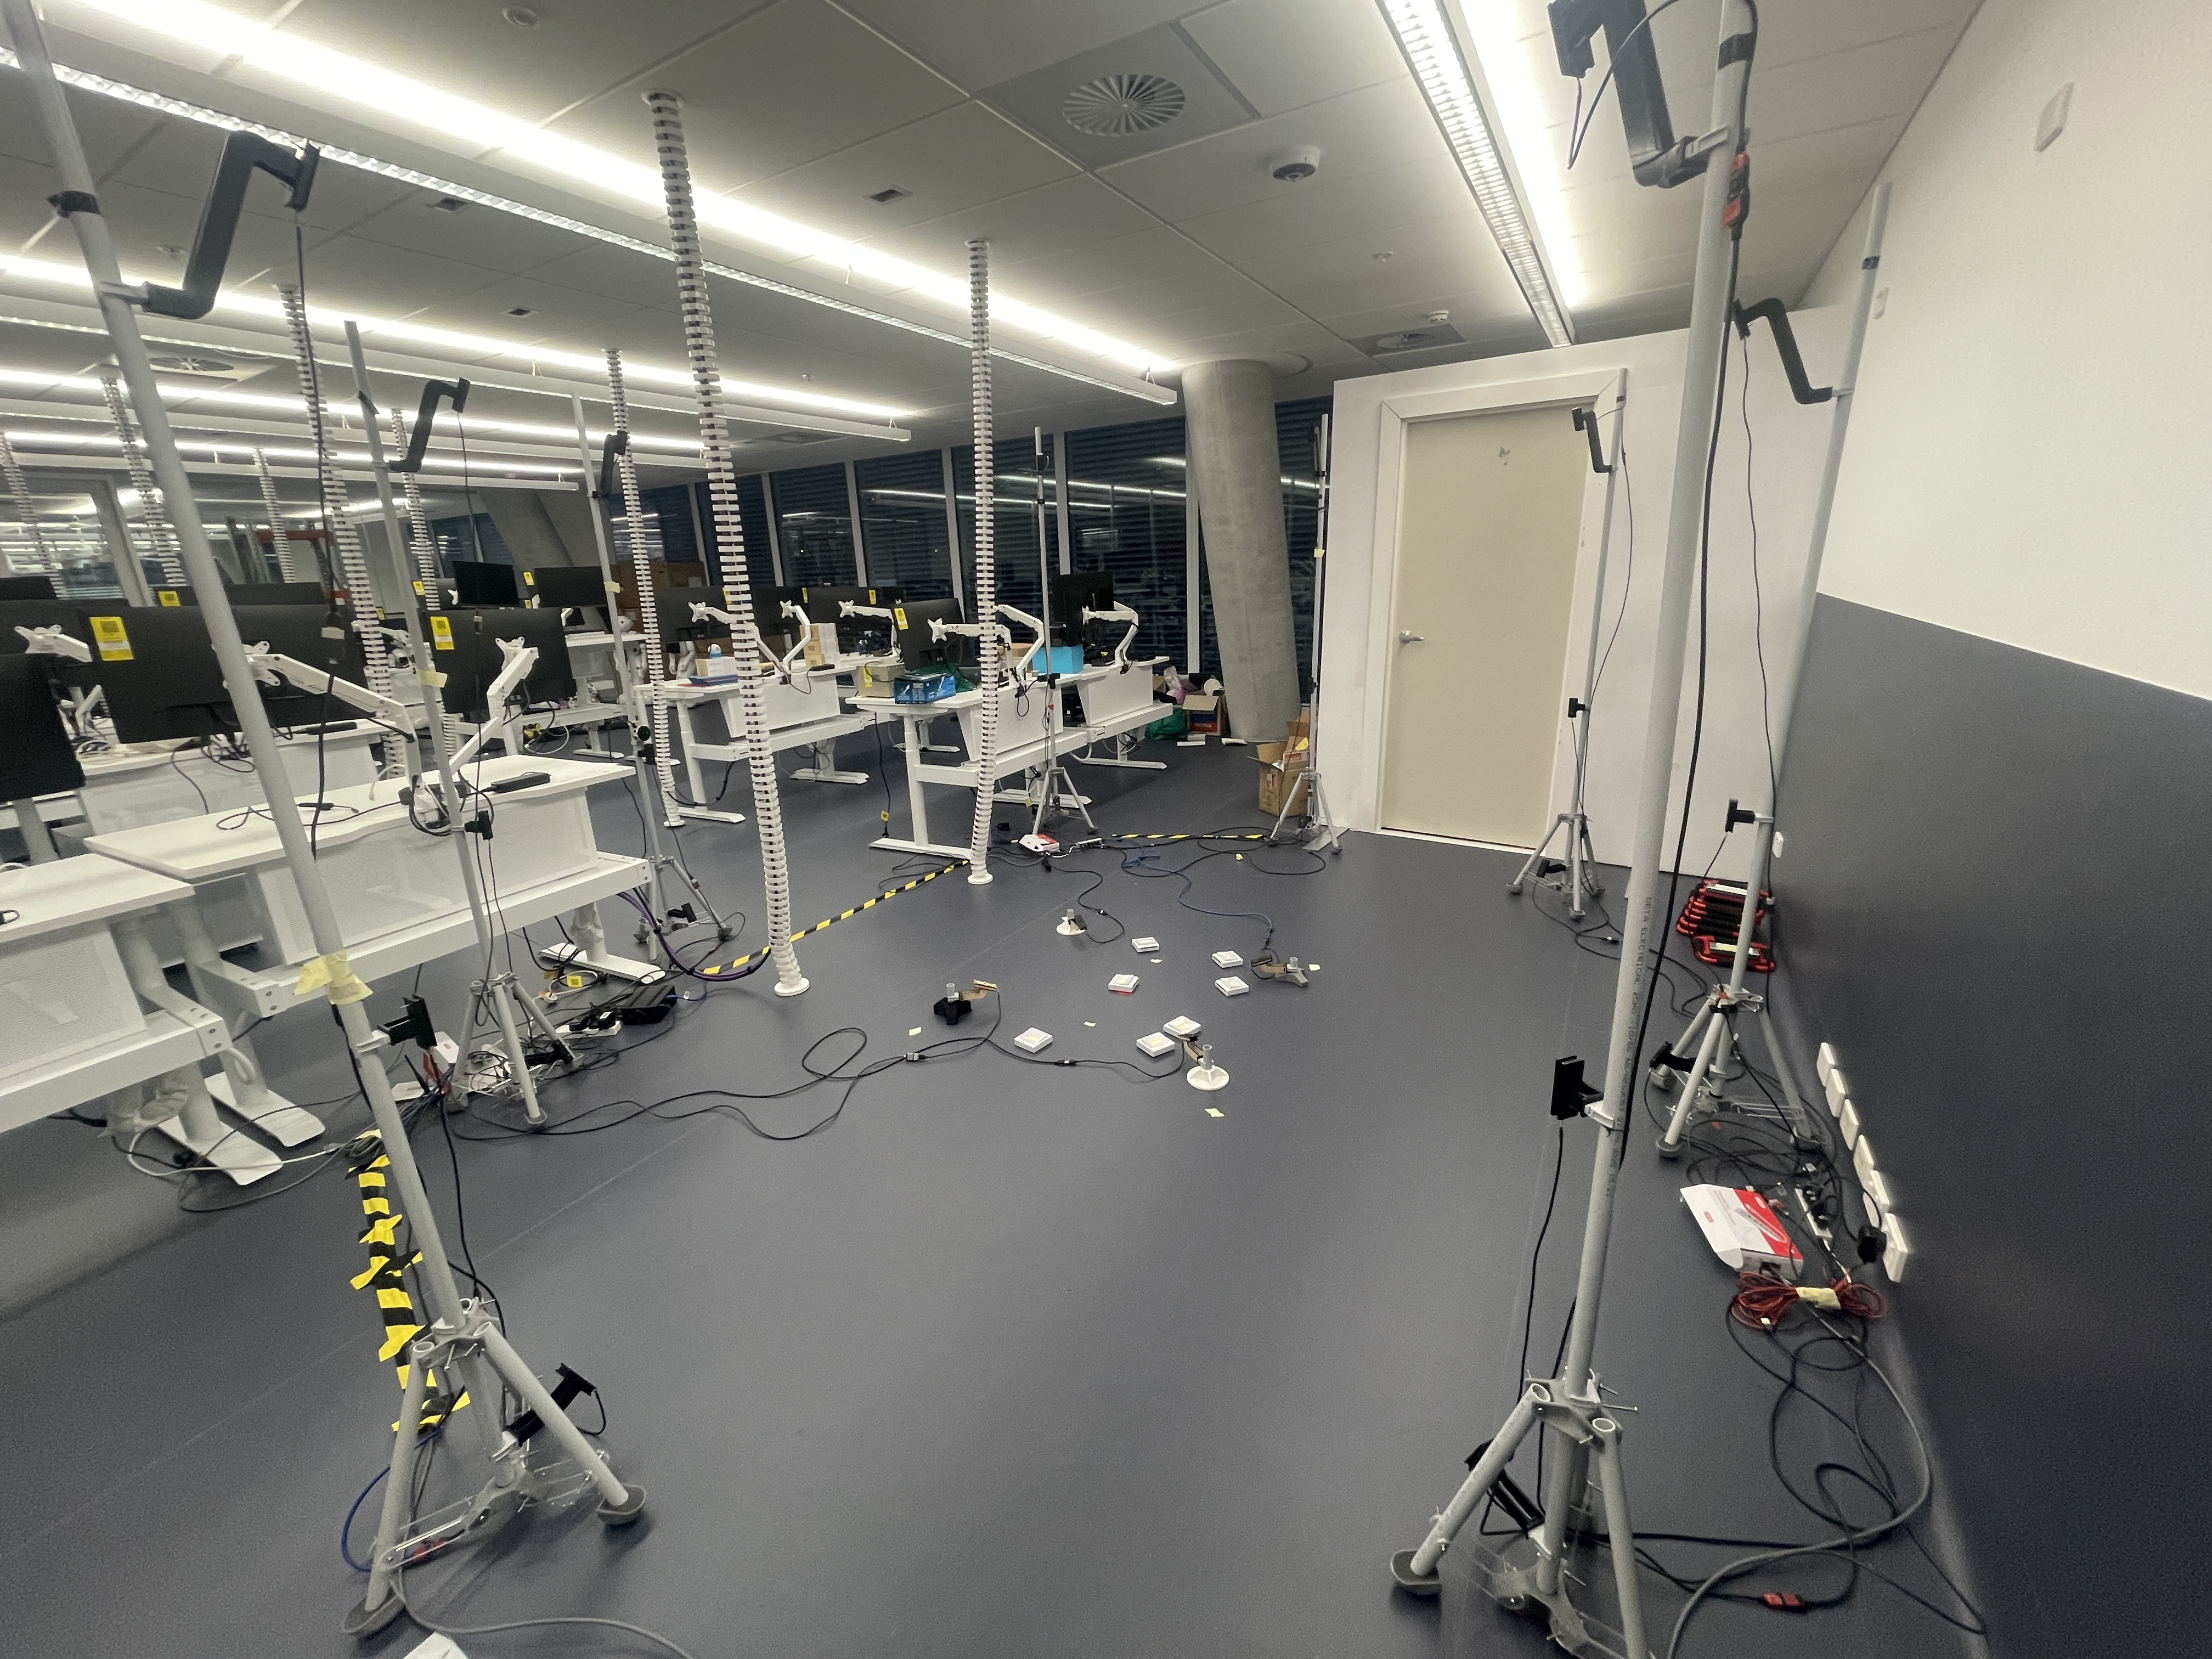
\includegraphics[width=0.85\textwidth]{IMG_5884.JPG} }}
  \caption{RIG scanning With Poles Locations}
  \label{fig:RIG}
\end{figure}

\newpage
\subsection{Cameras Calibration}
As mentioned before, there will be a set of twenty-eight camaras in the RIG. 
It is crucial to be able to calibrate these cameras an object the intrinsic parameters in order to input these parameters into the Photogrammetry Pipeline to enhance
the reconstruction process. The intrinsic parameters are illustrated in the camera  matrix on equation \ref{equ:camera_intrisics}.

All  the cameras were calibrated by taking a series of fifty photos of a checkerboard. In the images, the checker board is in different positions and orientation, as this enhances the calibration process.
Once all the images have been captures, these were processed using OpenCV and Matlab in order to perform the calibration process and obtain several paramaters such as the camera intrisics, distorsion, etc.

Table \ref{tab:Camera_Calibration} contains the result of the camera Calibration process for each camera.
% Please add the following required packages to your document preamble:
% \usepackage{graphicx}
\begin{table}[H]
  \centering
  \resizebox{\textwidth}{!}{%
  \begin{tabular}{|c|c|c|c|c|c|c|c|c|}
  \hline
  \textbf{Photo ID} &
    \textbf{Camera ID} &
    \textbf{Focal Lenght} &
    \textbf{Principal Point X} &
    \textbf{Principal Point y} &
    \textbf{Radial 1} &
    \textbf{Radial 2} &
    \textbf{FoV} &
    \textbf{ID} \\ \hline
  Lidar & Lidar & 1348.9      & 987.1289 & 552.4585 & 0.002083 & 0.004345 & 70 & 1  \\ \hline
  A1    & 23    & 2069.79669  & 1062.276 & 825.4553 & 0.043834 & -0.16655 & 65 & 2  \\ \hline
  A2    & 10    & 2023.979147 & 1055.148 & 740.4276 & 0.047799 & -0.18798 & 65 & 3  \\ \hline
  A3    & 14    & 2073.0703   & 1064.465 & 772.3883 & 0.037661 & -0.16921 & 65 & 4  \\ \hline
  A4    & 28    & 1685.622704 & 1044.281 & 772.533  & 0.056978 & -0.06307 & 65 & 5  \\ \hline
  A5    & 7     & 2077.408129 & 1054.39  & 849.7223 & 0.037899 & -0.19003 & 65 & 6  \\ \hline
  A6    & 20    & 2080.992114 & 1030.656 & 743.8521 & 0.043046 & -0.20511 & 65 & 7  \\ \hline
  A7    & 13    & 2035.145838 & 1070.591 & 764.946  & 0.025991 & -0.16304 & 65 & 8  \\ \hline
  A8    & 11    & 2057.82487  & 1025.147 & 799.6319 & 0.032882 & -0.14583 & 65 & 9  \\ \hline
  A9    & 4     & 2045.525031 & 1017.459 & 781.6747 & 0.052045 & -0.22293 & 65 & 10 \\ \hline
  B1    & 19    & 2007.968395 & 1053.849 & 793.203  & 0.040332 & -0.1859  & 65 & 11 \\ \hline
  B2    & 15    & 2031.574945 & 1060.078 & 775.8948 & 0.033055 & -0.17165 & 65 & 12 \\ \hline
  B3    & 3     & 2111.254725 & 1037.889 & 799.7706 & 0.032561 & -0.17198 & 65 & 13 \\ \hline
  B4    & 12    & 2058.9386   & 1022.306 & 742.7845 & 0.046652 & -0.20622 & 65 & 14 \\ \hline
  B5    & 2     & 2078.153107 & 980.6483 & 781.8416 & 0.060616 & -0.21788 & 65 & 15 \\ \hline
  B6    & 6     & 2099.600814 & 1000.535 & 731.1288 & 0.035295 & -0.20673 & 65 & 16 \\ \hline
  B7    & 16    & 2066.488622 & 1035.458 & 756.2719 & 0.045434 & -0.20259 & 65 & 17 \\ \hline
  B8    & 25    & 2076.530213 & 1060.421 & 815.187  & 0.06066  & -0.20289 & 65 & 18 \\ \hline
  B9    & 21    & 2031.68852  & 1038.411 & 743.4008 & 0.032986 & -0.19021 & 65 & 19 \\ \hline
  B10   & 26    & 2048.856969 & 1047.928 & 747.5051 & 0.037514 & -0.18331 & 65 & 20 \\ \hline
  C1    & 17    & 2072.818087 & 1037.388 & 805.2937 & 0.041437 & -0.17553 & 65 & 21 \\ \hline
  C2    & 9     & 2023.270233 & 1066.445 & 761.1484 & 0.039684 & -0.19295 & 65 & 22 \\ \hline
  C3    & 5     & 2038.942135 & 1052.651 & 734.7338 & 0.0562   & -0.2034  & 65 & 23 \\ \hline
  C4    & 8     & 2024.024741 & 1064.304 & 760.5158 & 0.037415 & -0.18791 & 65 & 24 \\ \hline
  C5    & 1     & 2063.919749 & 976.3176 & 761.5408 & 0.022828 & -0.11913 & 65 & 25 \\ \hline
  C6    & 22    & 2061.102003 & 1071.594 & 788.9326 & 0.053629 & -0.20935 & 65 & 26 \\ \hline
  C7    & 24    & 2060.07463  & 994.6496 & 772.853  & 0.053323 & -0.1899  & 65 & 27 \\ \hline
  C8    & 18    & 2124.144197 & 1060.398 & 822.0559 & 0.05472  & -0.25224 & 65 & 28 \\ \hline
  C9    & 27    & 2062.300912 & 995.6599 & 763.2463 & 0.045703 & -0.21291 & 65 & 29 \\ \hline
  \end{tabular}%
  }
  \caption{Cameras Calibration Parameters}
  \label{tab:Camera_Calibration}
  \end{table}

\subsection*{Execution}
The execution process starts by connecting the user computer to the Raspberry Pi's with a SSH connection via Putty.
Once a connection is established, a trial run will be performed to ensure the cameras are working as intended.
After the trial run is successful, the RIG is fully opertational.

Before a person enters the scan , the user is requirted to start the Nvidia Jetson Xavier and execute the Realsense SDK.
Once the mentioned above are perform, a person can enter the RIG to get scanned.
In parallel the administrator of the RIG will execute the script to capture data using putty. Once that script is executing, the administrator will take a Photo and PointCloud
using the RealSense SDK. 

The entire process takes approximately ten seconds. Once the data is captured, it can be used in the photogrammetry pipeline for reconstruction.




\chapter{Results}

\chapter{Conclusion}

\chapter{Recommendations}

\nocite{*}   % all not cited bib entrys are shown in bibliography ...
\bibliography{resources}


\appendix
\chapter{\vspace{-5.5cm}Appendix}

\begin{table}[!htb]
  \centering
  \makebox[\textwidth]
  {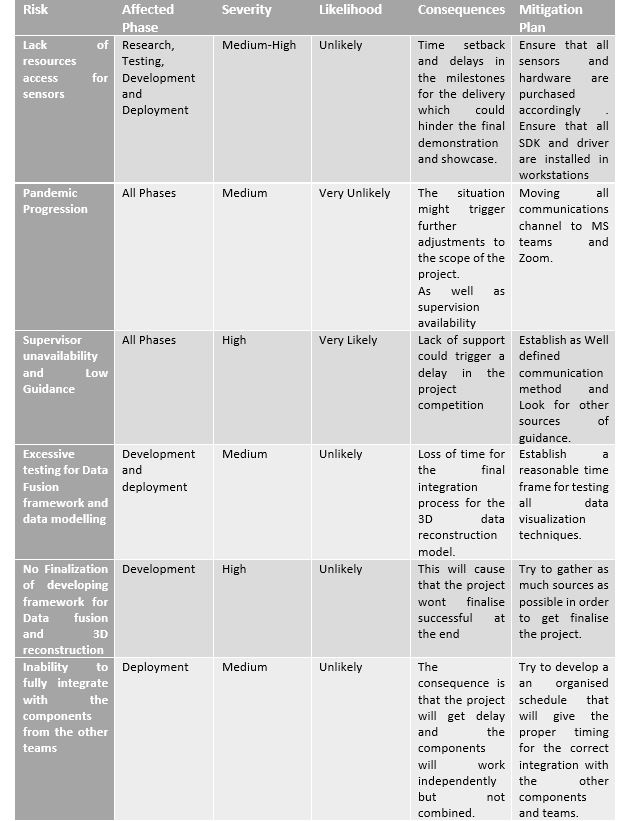
\includegraphics[width=1\linewidth]{Risk_matrix.png}    
  }
  \caption{Risk Matrix}
  \label{appendix:risk}
\end{table}

\newpage
\begin{table}
  \centering
  \makebox[\textwidth]
  {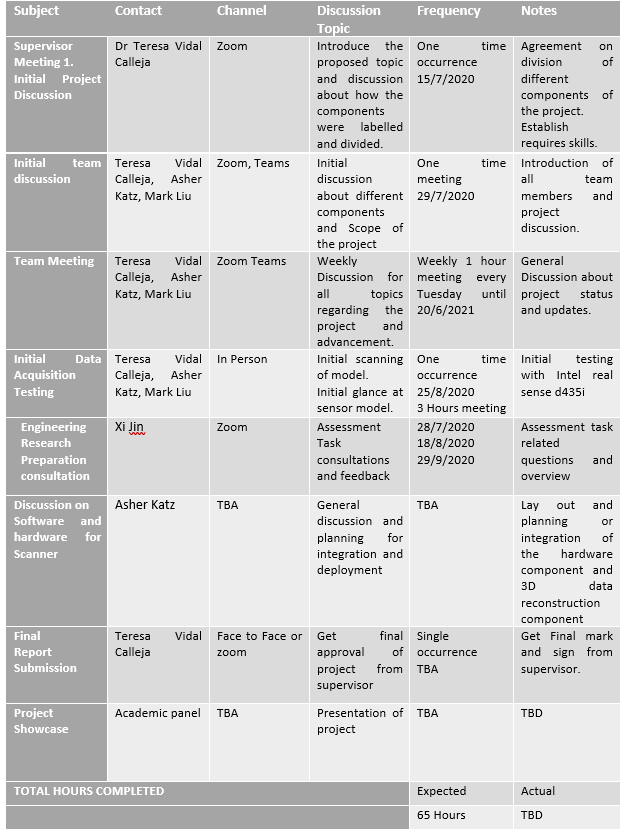
\includegraphics[width=1\linewidth]{ComunicationPlan.png}    
  }
  \caption{Comunication Plan}
  \label{appendix:ComunicationPlan}
  \end{table}    



\end{document}
